% Maximum Power Point Tracking as a Control Problem -- IEEE journal version.
% Build: tectonic -X compile journal.tex   (or pdfLaTeX + BibTeX on Overleaf)
\documentclass[journal]{IEEEtran}
\usepackage{amsmath,amssymb}
\usepackage{newtxtext,newtxmath}
\usepackage{graphicx,booktabs,cite,array}
\usepackage{siunitx}
\usepackage{xurl,needspace}
\usepackage{tikz}
\usetikzlibrary{arrows.meta,positioning,calc}
\usepackage[american,siunitx]{circuitikz}
\usepackage[hidelinks]{hyperref}
\raggedbottom
\setcounter{dbltopnumber}{2}
\renewcommand{\dbltopfraction}{0.85}
\renewcommand{\dblfloatpagefraction}{0.75}
\renewcommand{\topfraction}{0.85}
\renewcommand{\textfraction}{0.12}

\renewcommand{\IEEEQED}{}
\newtheorem{proposition}{Proposition}
\sisetup{per-mode=symbol}
\DeclareSIUnit\ohm{\ensuremath{\Omega}}
\DeclareSIUnit\celsius{\ensuremath{^{\circ}}C}
\DeclareSIUnit\degree{\ensuremath{^{\circ}}}
\DeclareSIUnit\percent{\ensuremath{\%}}

\newcommand{\vpv}{v_{\mathrm{pv}}}
\newcommand{\ipv}{i_{\mathrm{pv}}}
\newcommand{\Vmp}{V_{\mathrm{mp}}}
\newcommand{\Imp}{I_{\mathrm{mp}}}
\newcommand{\Pmp}{P_{\mathrm{mp}}}
\newcommand{\Voc}{V_{\mathrm{oc}}}
\newcommand{\Isc}{I_{\mathrm{sc}}}
\newcommand{\Wm}{\si{\watt\per\square\metre}}
\newcommand{\Wms}{\si{\watt\per\square\metre\per\second}}

\begin{document}
\title{Maximum Power Point Tracking as a Control Problem: Array-Dependent Damping, a Vanishing Loop Gain,
and Ramp-Robust Tracking}
\author{Ritesh~Roshan~Sahoo,
Arnav~Sharma,
Arushi~Uppal,
and~Krish~Sabharwal%
\thanks{The authors are with the Department of Artificial Intelligence and Data Science, Amrita School
of Artificial Intelligence, Amrita Vishwa Vidyapeetham, Faridabad, Haryana 121002, India.\protect\\
Corresponding author: R.~R.~Sahoo \protect\\ (e-mail: \mbox{riteshroshansahoo01@gmail.com}).}}
\markboth{}{Sahoo \MakeLowercase{\textit{et al.}}: Maximum Power Point Tracking as a Control Problem}
\maketitle

\begin{abstract}
Maximum power point tracking (MPPT) is usually studied as a search problem, with the converter that
carries it out treated as an ideal actuator. We study it as a feedback control problem, building one
verified chain from a module datasheet to a switched \SI{20}{\kilo\hertz} circuit for a
\SI{2.4}{\kilo\watt} photovoltaic array on a boost converter. Three results follow. First, the array's
dynamic resistance sets the damping of its own converter: along one I--V curve the resonance moves by under
\SI{4}{\percent} while the damping ratio changes by a factor of 44, from 0.023 to 1.035. A conventionally
tuned single proportional--integral voltage loop therefore develops three gain crossovers and its phase
margin falls to \SI{1.5}{\degree}, while a cascade with an inner current loop holds above \SI{85}{\degree}
at every operating point with one fixed set of gains. Second, the small-signal gain from duty ratio to
array power equals $\mathrm{d}P/\mathrm{d}V$ and is exactly zero at the optimum, which explains from first
principles why every tracker must estimate a gradient, and the measured \SI{11.9}{\milli\second} voltage-loop
settling time fixes the tracker period. Third, under identical inner loops on EN~50530-style irradiance
ramps, extremum seeking holds \SI{99.85}{\percent} efficiency at every rate from 25 to \SI{200}{\Wms},
while perturb and observe and incremental conductance fall to \SI{99.46}{\percent}; a variable-step perturb
and observe that wins the conventional step test collapses to \SI{93.14}{\percent} with a \SI{705}{\watt}
shortfall, because its adaptation law has positive feedback. A switched Simscape model agrees with the
averaged model to \SI{0.23}{\percent} in voltage and \SI{0.005}{\percent} in power. The pipeline is fully
scripted and covered by 27 unit tests.
\end{abstract}

\begin{IEEEkeywords}
Maximum power point tracking, photovoltaic systems, boost converter, cascade control, small-signal
modeling, extremum seeking control, perturb and observe, EN 50530, Simscape.
\end{IEEEkeywords}

\begin{figure*}[t]
\centering
\resizebox{\textwidth}{!}{%
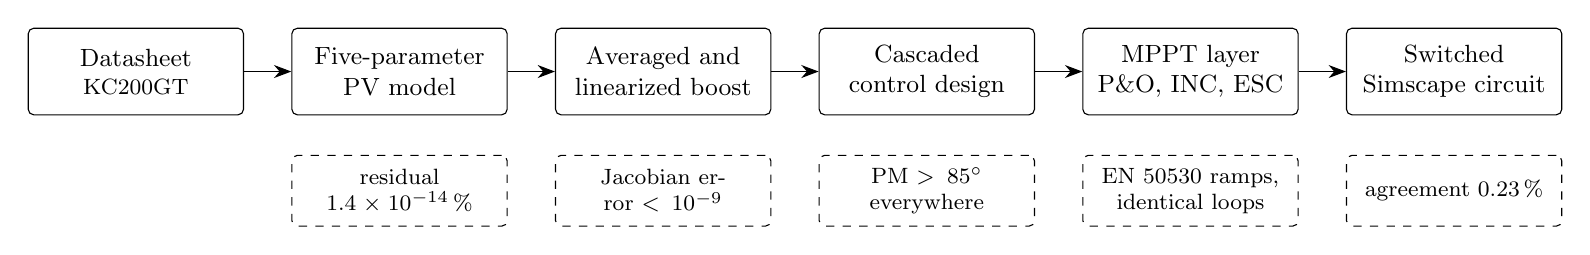
\begin{tikzpicture}[font=\small,
  stage/.style={draw, rounded corners=2pt, minimum height=11mm, text width=25mm, align=center},
  chk/.style={draw, dashed, rounded corners=2pt, minimum height=9mm, text width=25mm, align=center, font=\footnotesize},
  >={Stealth[length=2.2mm]}]
\node[stage] (a) {Datasheet\\[-1pt]\footnotesize KC200GT};
\node[stage, right=6mm of a] (b) {Five-parameter\\ PV model};
\node[stage, right=6mm of b] (c) {Averaged and\\ linearized boost};
\node[stage, right=6mm of c] (d) {Cascaded\\ control design};
\node[stage, right=6mm of d] (e) {MPPT layer\\ P\&O, INC, ESC};
\node[stage, right=6mm of e] (f) {Switched\\ Simscape circuit};
\foreach \x/\y in {a/b,b/c,c/d,d/e,e/f} \draw[->] (\x) -- (\y);
\node[chk, below=5mm of b] {residual $1.4\times10^{-14}\,\%$};
\node[chk, below=5mm of c] {Jacobian error $<10^{-9}$};
\node[chk, below=5mm of d] {PM $>\SI{85}{\degree}$ everywhere};
\node[chk, below=5mm of e] {EN 50530 ramps, identical loops};
\node[chk, below=5mm of f] {agreement \SI{0.23}{\percent}};
\end{tikzpicture}}
\caption{The verification chain of this paper. Each stage (solid) is checked against something that does
not share its assumptions (dashed) before the next stage depends on it.}
\label{fig:chain}
\end{figure*}

\section{Introduction}
\IEEEPARstart{A}{} \SI{2.4}{\kilo\watt} array of twelve Kyocera KC200GT modules~\cite{kyocera} delivers
its rated power at one terminal voltage, \SI{157.8}{\volt} at \SI{1000}{\Wm} and \SI{25}{\celsius}. That
point moves: the available power falls from \SI{2402}{\watt} to \SI{478}{\watt} as irradiance drops to
\SI{200}{\Wm}, and a \SI{40}{\kelvin} change in cell temperature shifts the optimum voltage by nearly
\SI{30}{\volt}. Maximum power point tracking (MPPT) keeps the array at that moving optimum using only
terminal measurements, by adjusting the duty ratio of a DC--DC converter.

The literature mostly treats MPPT as a search problem: which rule finds the peak fastest~\cite{esram}.
That framing leaves three gaps. Panel models are validated at the datasheet points~\cite{villalva}, yet
the controller depends on the slope $\mathrm{d}I/\mathrm{d}V$, which those points do not constrain.
Tracker periods, steps and gains are tuned by trial, although they are set by the converter
loop~\cite{femia}. And benchmarks use step changes far more often than the standard ramp
profiles~\cite{en50530}, so trackers that fail on ramps go unnoticed.

We ask: \emph{if MPPT is treated as a feedback control problem, with a verified plant, quantified
margins and a standard dynamic benchmark, which control structure and which tracker keep the array
closest to maximum power, and why?} We answer it with one verified chain (Fig.~\ref{fig:chain}) and make
five contributions.
\begin{enumerate}
\item A datasheet-only five-parameter model whose slope, not only its operating points, is verified,
identified to machine precision (Sections~\ref{sec:pv} and~\ref{sec:res-pv}).
\item An explicit small-signal plant showing that the array's dynamic resistance sets the converter's
damping, which varies $44\times$ along one I--V curve, and a proof that the duty-to-power gain vanishes at
the optimum (Sections~\ref{sec:plant} and~\ref{sec:res-plant}).
\item A margin analysis over the whole operating envelope showing that a single PI loop is structurally
unsafe and a cascade is not (Sections~\ref{sec:control} and~\ref{sec:res-control}).
\item A fair benchmark of four trackers under identical inner loops on step and EN~50530-style ramp tests,
including a documented instability of variable-step perturb and observe (Section~\ref{sec:res-mppt}).
\item A switched Simscape model with a native photovoltaic component that validates the averaged model,
and a reproducible pipeline with 27 unit tests (Sections~\ref{sec:switched} and~\ref{sec:res-switched}).
\end{enumerate}

\section{Related Work}
\label{sec:related}
\emph{Device models.} The single-diode model is settled; its parameterization is not. Villalva
\emph{et al.}~\cite{villalva} fix the ideality factor and iterate on the series resistance, leaving the
open-circuit temperature coefficient unused. De Soto \emph{et al.}~\cite{desoto} close the system with that
coefficient, at the cost of a badly scaled solve. Few studies check the slope away from the imposed points.

\emph{Trackers.} Esram and Chapman~\cite{esram} survey nineteen methods as search procedures. Femia
\emph{et al.}~\cite{femia,femia_book} show that the perturb and observe (P\&O) period must exceed the
converter settling time. Incremental conductance (INC)~\cite{hussein} is often claimed superior, but Sera
\emph{et al.}~\cite{sera} and Elgendy \emph{et al.}~\cite{elgendy} find the two equivalent under equal
implementation. Extremum seeking control (ESC) rests on averaging theory~\cite{krstic,ariyur} and was
applied to photovoltaics by Leyva \emph{et al.}~\cite{leyva}; ripple correlation control~\cite{rcc} uses
the switching ripple as the dither. Global methods for partial shading~\cite{nguyen} are orthogonal to
this work.

\emph{Converter control.} State-space averaging~\cite{middlebrook,erickson} is standard. The boost
converter's right-half-plane zero lies on the duty-to-output path, not the input path a tracker regulates.
Cascaded control of photovoltaic converters is established~\cite{bratcu,kjaer}, but tracking studies
rarely state crossover or margin, or whether they hold elsewhere on the curve.

What these lines of work share is that none connects panel curvature, converter dynamics and tracker
tuning into one verified chain. Table~\ref{tab:related} positions this paper.

\begin{table}[!t]
\centering
\caption{Positioning Against Representative Prior Work}
\label{tab:related}
\footnotesize
\setlength{\tabcolsep}{3pt}
\begin{tabular}{@{}>{\raggedright}p{0.24\columnwidth}>{\raggedright}p{0.32\columnwidth}>{\raggedright\arraybackslash}p{0.38\columnwidth}@{}}
\toprule
Work & Covers & Left open \\
\midrule
\cite{villalva} & Robust extraction & Ideality assumed; slope unverified \\
\cite{desoto} & Determined extraction & Conditioning; no control use \\
\cite{esram} & Survey of 19 trackers & Converter dynamics out of scope \\
\cite{femia} & Period from settling & No envelope-wide margins \\
\cite{sera} & P\&O vs.\ INC, equal setup & No ramps, no ESC \\
\cite{leyva} & ESC design for PV & No standard ramp comparison \\
\cite{bratcu} & Cascaded PV converters & Margins not swept along I--V \\
\midrule
This work & Datasheet to switched circuit, each link verified & Shading, sensor noise, hardware \\
\bottomrule
\end{tabular}
\end{table}

\section{System and Models}
\label{sec:models}

\subsection{System Under Study}
The array is six KC200GT modules in series by two strings in parallel, \SI{2402}{\watt} at standard test
conditions (STC), with its maximum power point (MPP) at \SI{157.8}{\volt}, \SI{15.22}{\ampere}. A boost
converter with $L=\SI{1.5}{\milli\henry}$, $R_L=\SI{0.15}{\ohm}$, $C_{\mathrm{pv}}=\SI{100}{\micro\farad}$
and $f_{sw}=\SI{20}{\kilo\hertz}$ feeds a stiff \SI{400}{\volt} bus. The inductor gives \SI{20}{\percent}
current ripple at the STC MPP and the capacitor keeps voltage ripple below \SI{0.25}{\volt}; the LC corner of
\SI{411}{\hertz} is well below $f_{sw}/10$, as averaging requires.

\subsection{Photovoltaic Model}
\label{sec:pv}
Each module obeys the single-diode equation
\begin{equation}
I = I_{ph} - I_0\!\left[e^{(V + I R_s)/a} - 1\right] - \frac{V + I R_s}{R_{sh}},\quad a = \frac{n N_s k T_c}{q},
\label{eq:sd}
\end{equation}
translated to other conditions with the De Soto relations~\cite{desoto}. The five unknowns are fixed by
five STC conditions: $I(0)=\Isc$, $I(\Voc)=0$, $I(\Vmp)=\Imp$, stationarity
$\Imp + \Vmp\,\mathrm{d}I/\mathrm{d}V|_{\Vmp}=0$, and $\mathrm{d}\Voc/\mathrm{d}T=\beta_{Voc}$. The
stationarity condition pins the slope at the MPP, which fixes the curvature the controller depends on; the
temperature condition makes the ideality factor an output that can be checked against physics. The system is
solved by a trust-region method on $[I_{ph},\ln I_0,\ln R_s,\ln R_{sh},n]$ with scaled residuals and six
ideality seeds. Current is found from~\eqref{eq:sd} by damped Newton iteration, which converges
monotonically from $I=0$ because the residual is decreasing and concave, and warm starting reduces each solve
to two or three iterations. The slope is analytic:
\begin{equation}
\frac{\mathrm{d}I}{\mathrm{d}V} = -\frac{g_d + 1/R_{sh}}{1 + R_s g_d + R_s/R_{sh}},\qquad
g_d = \frac{I_0}{a}e^{(V+IR_s)/a},
\label{eq:didv}
\end{equation}
and the dynamic resistance is $r_d = -(\mathrm{d}I/\mathrm{d}V)^{-1}$, which equals $\Vmp/\Imp$ at the MPP.

\subsection{Converter Plant}
\label{sec:plant}
With states $\vpv$ and $i_L$, the averaged boost model is
\begin{equation}
C_{\mathrm{pv}}\dot v_{\mathrm{pv}} = \ipv(\vpv) - i_L,\qquad
L\,\dot i_L = \vpv - (1-d)V_{dc} - R_L i_L .
\label{eq:avg}
\end{equation}
Linearizing about $(V,I,D)$ with $g=\mathrm{d}I/\mathrm{d}V$ gives
\begin{equation}
G_{vd}(s) = \frac{-V_{dc}/(LC_{\mathrm{pv}})}{s^2 + \left(\frac{R_L}{L} + \frac{1}{r_d C_{\mathrm{pv}}}\right)s + \frac{1-gR_L}{LC_{\mathrm{pv}}}} .
\label{eq:gvd}
\end{equation}
Three properties follow. The numerator is constant, so the duty-to-input-voltage path has no zero; the
boost converter's non-minimum-phase behavior lives on the output path only. The gain is negative: raising $d$
lowers $\vpv$. And the natural frequency $\omega_n\approx 1/\sqrt{LC_{\mathrm{pv}}}$ is fixed by the passive
parts, while the damping
\begin{equation}
2\zeta\omega_n = \frac{R_L}{L} + \frac{1}{r_d C_{\mathrm{pv}}}
\label{eq:zeta}
\end{equation}
is inversely proportional to $r_d$. The array is the damping element of its own converter.

\begin{proposition}[Vanishing loop gain]
\label{prop:vanish}
The DC gain from duty ratio to array power is
\begin{equation}
\left.\frac{\partial P}{\partial d}\right|_{DC} = \frac{\mathrm{d}P}{\mathrm{d}V}\cdot\frac{-V_{dc}}{1-gR_L},
\label{eq:pgain}
\end{equation}
which is zero at the MPP and changes sign across it.
\end{proposition}
\begin{IEEEproof}
The linearized power output is $\delta P = (I+Vg)\,\delta v = (\mathrm{d}P/\mathrm{d}V)\,\delta v$, and the DC
value of~\eqref{eq:gvd} is $-V_{dc}/(1-gR_L)$. At the MPP $\mathrm{d}P/\mathrm{d}V=0$.
\end{IEEEproof}

No fixed linear controller can therefore regulate power to its extremum. The MPPT layer must estimate the
gradient, which is what every tracker in Section~\ref{sec:mppt} does.

\section{Control Design}
\label{sec:control}
Because the MPPT layer and the weather choose the operating point, one fixed set of gains must hold
margins across the whole curve. Two structures were designed by loop shaping on simplified models and then
verified on the full-order plant (Fig.~\ref{fig:cascade}).

\begin{figure}[t]
\centering
\resizebox{\columnwidth}{!}{%
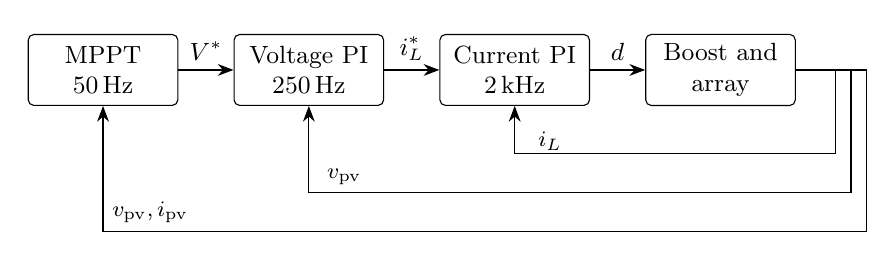
\begin{tikzpicture}[font=\small,
  box/.style={draw, rounded corners=2pt, minimum height=9mm, minimum width=19mm, align=center},
  >={Stealth[length=2mm]}]
\node[box] (m) {MPPT\\ \SI{50}{\hertz}};
\node[box, right=7mm of m] (v) {Voltage PI\\ \SI{250}{\hertz}};
\node[box, right=7mm of v] (i) {Current PI\\ \SI{2}{\kilo\hertz}};
\node[box, right=7mm of i] (p) {Boost and\\ array};
\draw[->] (m) -- node[above]{$V^\ast$} (v);
\draw[->] (v) -- node[above]{$i_L^\ast$} (i);
\draw[->] (i) -- node[above]{$d$} (p);
\draw[->] ($(p.east)+(0,0)$) -- ++(5mm,0) |- ($(i.south)+(0,-6mm)$) -| (i.south);
\draw[->] ($(p.east)+(5mm,0)$) -- ++(2mm,0) |- ($(v.south)+(0,-11mm)$) -| (v.south);
\draw[->] ($(p.east)+(7mm,0)$) -- ++(2mm,0) |- ($(m.south)+(0,-16mm)$) -| (m.south);
\node[font=\footnotesize] at ($(i.south)+(0.45,-0.45)$) {$i_L$};
\node[font=\footnotesize] at ($(v.south)+(0.45,-0.9)$) {$\vpv$};
\node[font=\footnotesize] at ($(m.south)+(0.6,-1.35)$) {$\vpv,\ipv$};
\end{tikzpicture}}
\caption{Three-layer cascade separated by timescale; each layer runs about eight times slower than the one
below.}
\label{fig:cascade}
\end{figure}

\emph{Single-loop baseline.} One PI acts on the voltage error and outputs the duty ratio, with crossover at
\SI{130}{\hertz} and its zero at \SI{26}{\hertz}, giving $K_p = 2.264\times10^{-3}$ and $K_i = 0.370$ at the
STC MPP.

\emph{Cascade.} The duty-to-current transfer
\begin{equation}
G_{id}(s) = \frac{V_{dc}}{L}\,\frac{s - g/C_{\mathrm{pv}}}{\Delta(s)} \approx \frac{V_{dc}}{Ls}\quad(\omega\gg\omega_n)
\end{equation}
is independent of the operating point above the resonance, so an inner loop at \SI{2}{\kilo\hertz} gets
$K_{p,i} = L\omega_{ci}/V_{dc} = 0.04712$ and $K_{i,i} = 59.2$. With the inner loop closed, the outer plant
is $-1/(C_{\mathrm{pv}}s + 1/r_d)$, with no resonance, and at \SI{250}{\hertz} it gives
$K_{p,v} = C_{\mathrm{pv}}\omega_{cv} = 0.15708$ and $K_{i,v} = 49.35$. Both loops are re-analyzed on the
exact plant with $L_v = -C_v G_{vd} C_i/(1 + C_i G_{id})$, and both include back-calculation anti-windup.

\emph{Tracker period.} A hill climber must wait for the voltage loop to settle before it judges its last
move. The measured settling time is \SI{11.9}{\milli\second}, so the period is \SI{20}{\milli\second}.

\section{Tracking Algorithms and Benchmark}
\label{sec:mppt}
All trackers derive from one abstract class that owns clamping, limits and timing, and drive the same
plant and cascade. P\&O moves the reference by $\pm\Delta V$ and reverses whenever power falls; it cycles
with peak-to-peak amplitude $2\Delta V$. A variable-step P\&O scales the step with $|\Delta P/\Delta V|$
within \SIrange{0.25}{6}{\volt}. INC~\cite{hussein} follows the sign of
$\Delta I/\Delta V + I/V = V^{-1}\mathrm{d}P/\mathrm{d}V$. ESC adds a dither $A\sin\omega t$, removes the DC part
of power with a washout, demodulates and integrates:
$\dot{\hat V} = K\,\mathrm{LPF}[\xi\sin\omega t] \approx K(A/2)\,\mathrm{d}P/\mathrm{d}V$. We use
$A=\SI{3}{\volt}$, \SI{25}{\hertz}, \SI{5}{\hertz} filter corners and $K=20$; ESC runs at
\SI{200}{\micro\second} and the hill climbers at \SI{20}{\milli\second}. P\&O and INC use
$\Delta V = \SI{1.5}{\volt}$.

Three signal classes are used: constant irradiance (steady-state cost), a \SIrange{1000}{500}{\Wm} step, and
trapezoidal ramps between 300 and \SI{1000}{\Wm} at 25, 50, 100 and \SI{200}{\Wms} with \SI{1}{\second}
dwells, following the medium-to-high class of EN~50530~\cite{en50530}. We use one up-down cycle per slope,
and the fastest rate lies above the standard's range by design. The figure of merit is
\begin{equation}
\eta_{\mathrm{MPPT}} = \int_{t_0}^{t_1}\vpv\ipv\,\mathrm{d}t \Big/ \int_{t_0}^{t_1}\Pmp\big(G(t)\big)\,\mathrm{d}t ,
\label{eq:eta}
\end{equation}
with the exact MPP solved on 240 irradiance values and interpolated, the first second excluded, and the
worst instantaneous shortfall reported alongside.

\section{Switched Circuit Model}
\label{sec:switched}
To audit the averaging assumption, the panel was written as a native Simscape component whose
constitutive law is~\eqref{eq:sd}, so the solver handles the implicit equation and no algebraic loop arises.
The boost stage uses only Foundation Library blocks with an ideal switch driven by a \SI{20}{\kilo\hertz}
sawtooth comparator, and a one-sample delay models the computation latency of a digital controller; at
\SI{50}{\micro\second} it costs about \SI{36}{\degree} at the inner crossover, which the design margin
absorbs (Fig.~\ref{fig:slx}).

\begin{figure}[t]
\centering
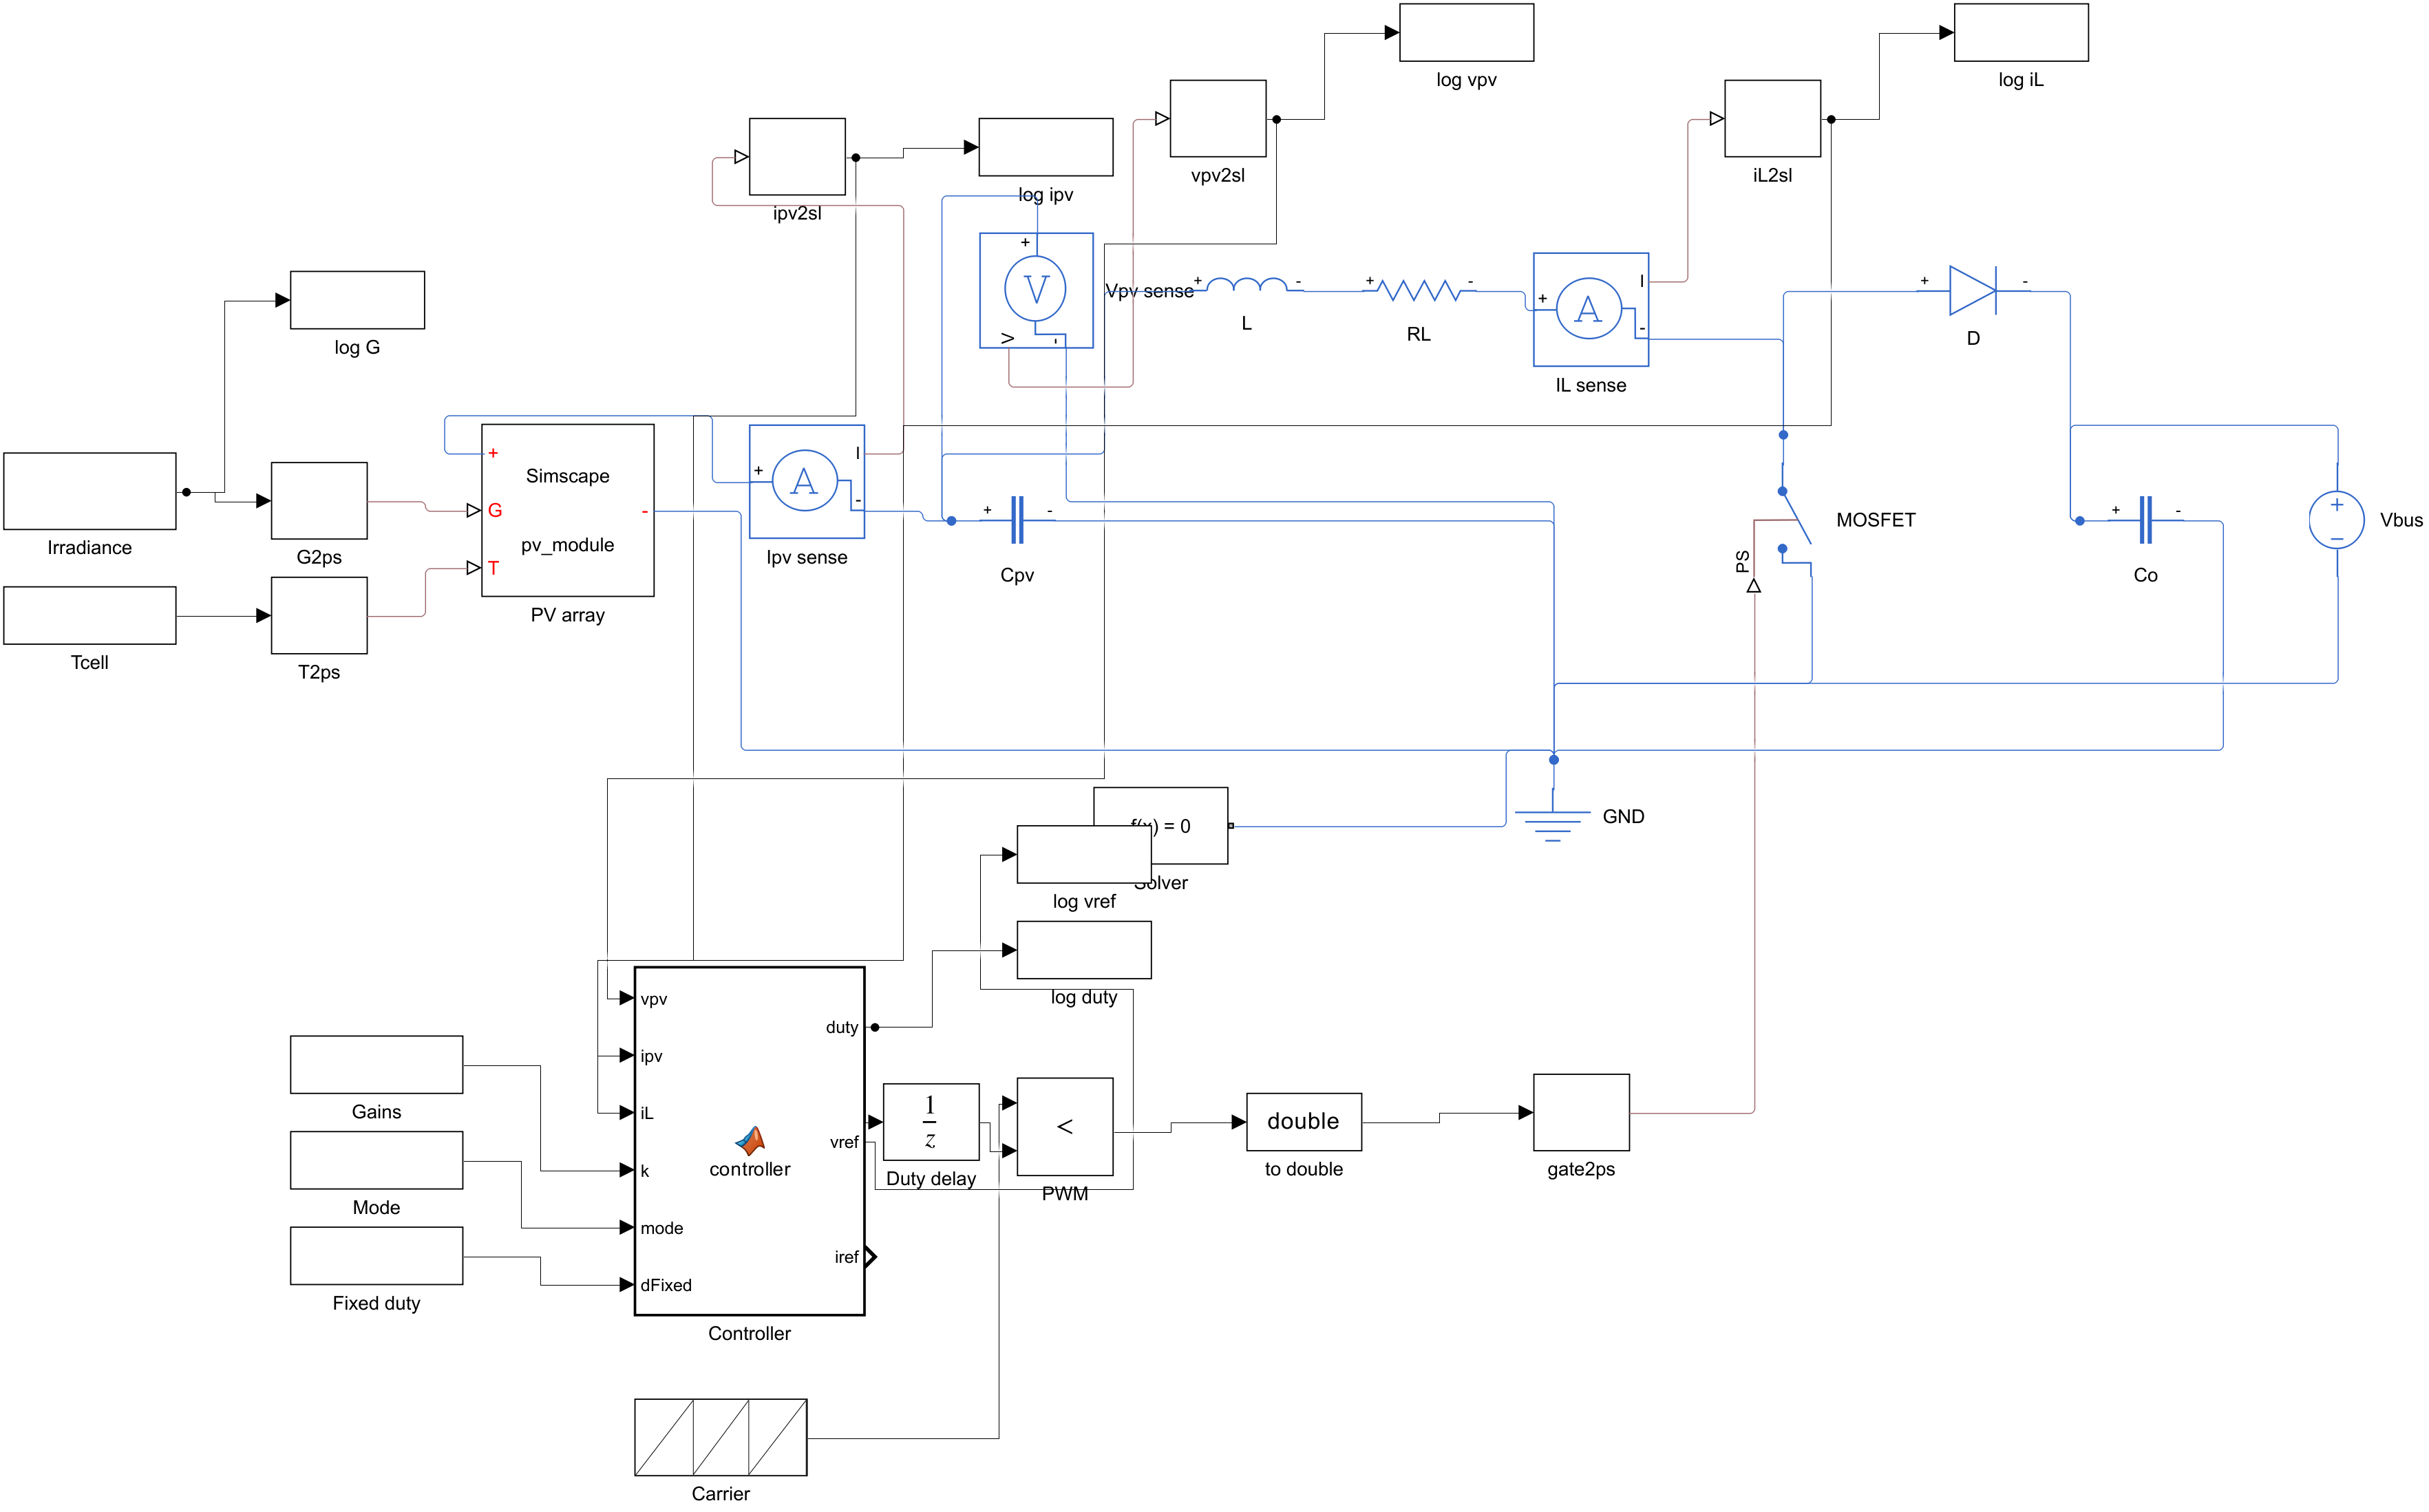
\includegraphics[width=\columnwidth]{figures/s07_simulink_model.png}
\caption{Switched Simulink and Simscape model: photovoltaic component (left), boost stage with sensing
(center), discrete cascade with one-sample delay and PWM comparator (bottom).}
\label{fig:slx}
\end{figure}

\section{Results}
\label{sec:results}

\subsection{Photovoltaic Model}
\label{sec:res-pv}
All five constraints are met to machine precision (Table~\ref{tab:pv}); the worst error is
$1.4\times10^{-14}\,\%$ and the extracted ideality factor is $n=1.0036$, physically sensible for crystalline
silicon. The analytic slope matches a central difference to below $10^{-5}$ over $0.05\Voc$ to $0.97\Voc$,
and the method converges on a 96-cell SunPower SPR-305E with a worst error of $7\times10^{-11}\,\%$.
Fig.~\ref{fig:pv} shows that $\Vmp$ moves only \SIrange{156.0}{159.2}{\volt} over a fivefold irradiance
change, whereas $r_d$ spans from under \SI{2}{\ohm} near $\Voc$ to nearly \SI{500}{\ohm} on the
current-source branch.

\begin{table}[!t]
\centering
\caption{Identified KC200GT Parameters and Datasheet Agreement at STC}
\label{tab:pv}
\footnotesize
\begin{tabular}{@{}lr@{\hspace{14pt}}lrr@{}}
\toprule
Parameter & Value & Quantity & Datasheet & Error (\%) \\
\midrule
$I_{ph}$ (A) & 8.22713 & $\Voc$ (V) & 32.90 & 0 \\
$I_0$ (A) & $4.3964\times10^{-10}$ & $\Isc$ (A) & 8.21 & 0 \\
$R_s$ ($\Omega$) & 0.33501 & $\Vmp$ (V) & 26.30 & $-1.4\times10^{-14}$ \\
$R_{sh}$ ($\Omega$) & 160.6015 & $\Imp$ (A) & 7.61 & 0 \\
$a$ (V) & 1.39246 & $\Pmp$ (W) & 200.14 & 0 \\
$n$ & 1.0036 & $\beta_{Voc}$ (V/K) & $-0.12301$ & $1.1\times10^{-14}$ \\
\bottomrule
\end{tabular}
\end{table}

\begin{figure}[!t]
\centering
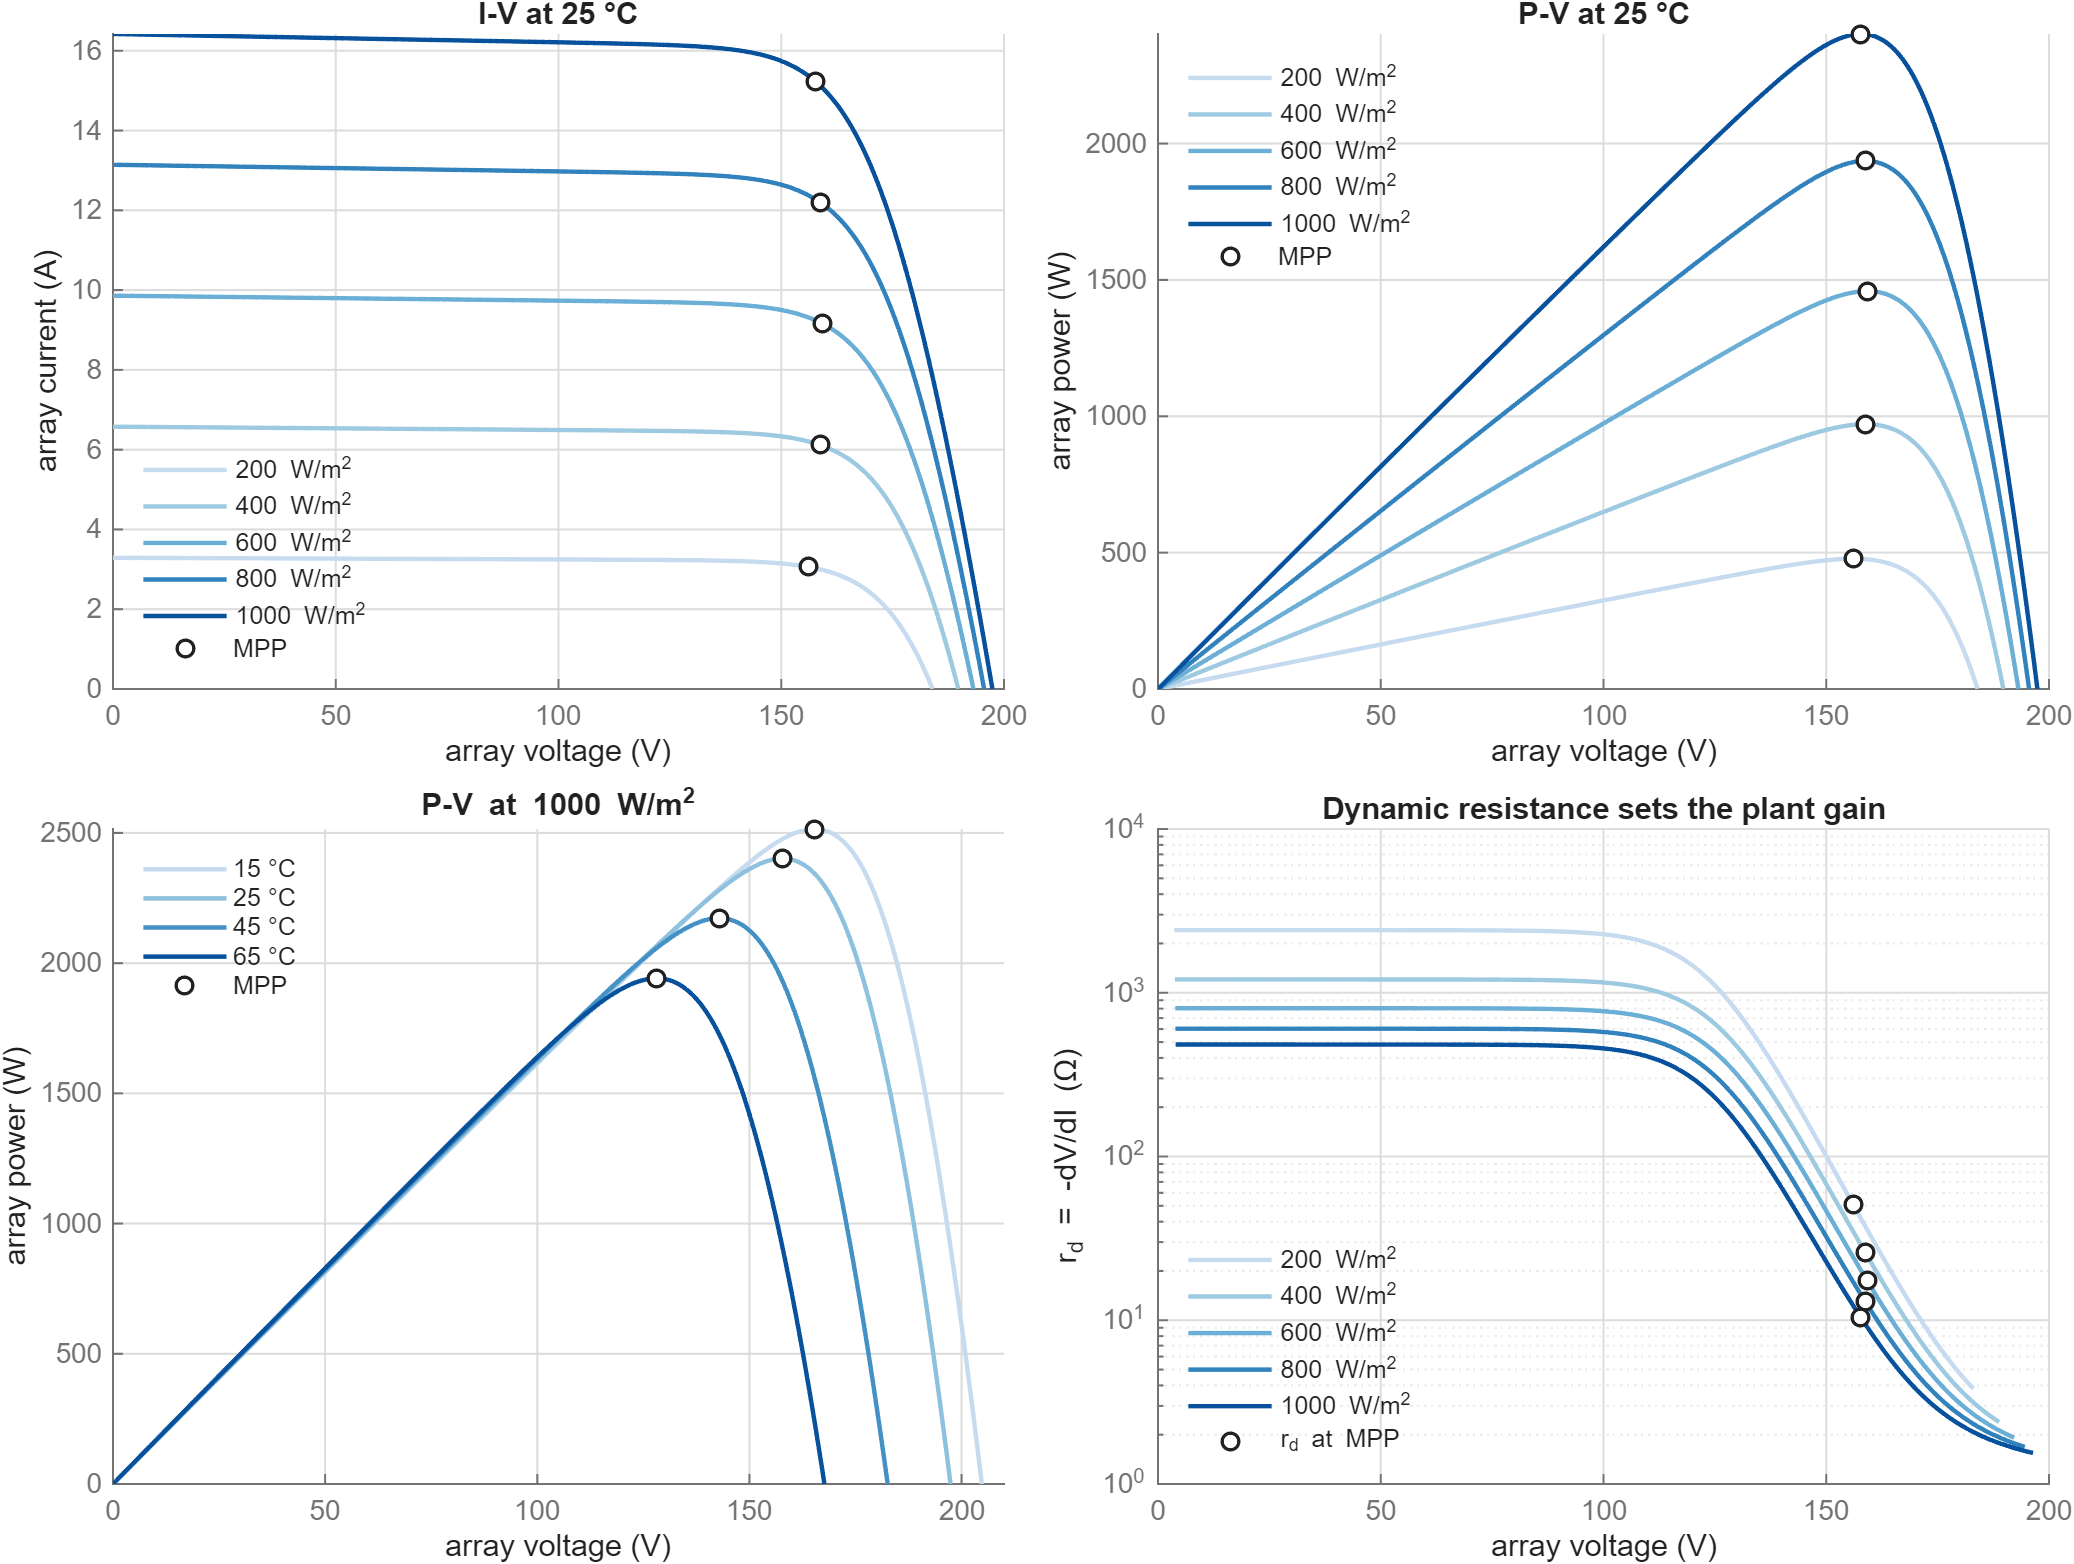
\includegraphics[width=\columnwidth]{figures/s01_pv_characteristics.png}
\caption{Characteristics of the $6\times2$ KC200GT array: I--V and P--V curves at \SI{25}{\celsius} (top),
effect of temperature at \SI{1000}{\Wm} (bottom left), and dynamic resistance $r_d$ on a log axis (bottom
right).}
\label{fig:pv}
\end{figure}

\subsection{Plant Across the Operating Envelope}
\label{sec:res-plant}
Along one I--V curve at \SI{1000}{\Wm} the resonance moves by under \SI{4}{\percent} while $\zeta$ changes
$44\times$ (Table~\ref{tab:env}), confirming~\eqref{eq:zeta}. The resonance peak reaches about
\SI{27}{\decibel} on the current-source branch and almost vanishes near $\Voc$ (Fig.~\ref{fig:bode}). The
duty-to-current response is the same at all points above a few hundred hertz, which is what makes the inner
loop easy. The duty-to-power gain at the MPP evaluates to $8.9\times10^{-15}$\,W, zero to round-off, as
Proposition~\ref{prop:vanish} predicts. The converter stays in continuous conduction down to \SI{200}{\Wm},
where the mean current is 1.93 times half the ripple.

\begin{table}[!t]
\centering
\caption{Small-Signal Plant Along the I--V Curve at 1000~W/m$^2$}
\label{tab:env}
\footnotesize
\begin{tabular}{@{}rrrrrr@{}}
\toprule
$V$ (V) & $V/\Voc$ & $r_d$ ($\Omega$) & $f_n$ (Hz) & $\zeta$ & $\mathrm{d}P/\mathrm{d}V$ (W/V) \\
\midrule
69.09 & 0.35 & 482.1 & 411.0 & 0.0234 & $+16.13$ \\
108.57 & 0.55 & 417.6 & 411.0 & 0.0240 & $+15.93$ \\
138.18 & 0.70 & 77.23 & 411.3 & 0.0444 & $+14.25$ \\
157.80 & 0.799 & 10.37 & 413.9 & 0.2047 & $\approx 0$ \\
173.71 & 0.88 & 3.077 & 420.8 & 0.6335 & $-44.40$ \\
187.53 & 0.95 & 1.832 & 427.4 & 1.0350 & $-96.41$ \\
\bottomrule
\end{tabular}
\end{table}

\begin{figure}[!t]
\centering
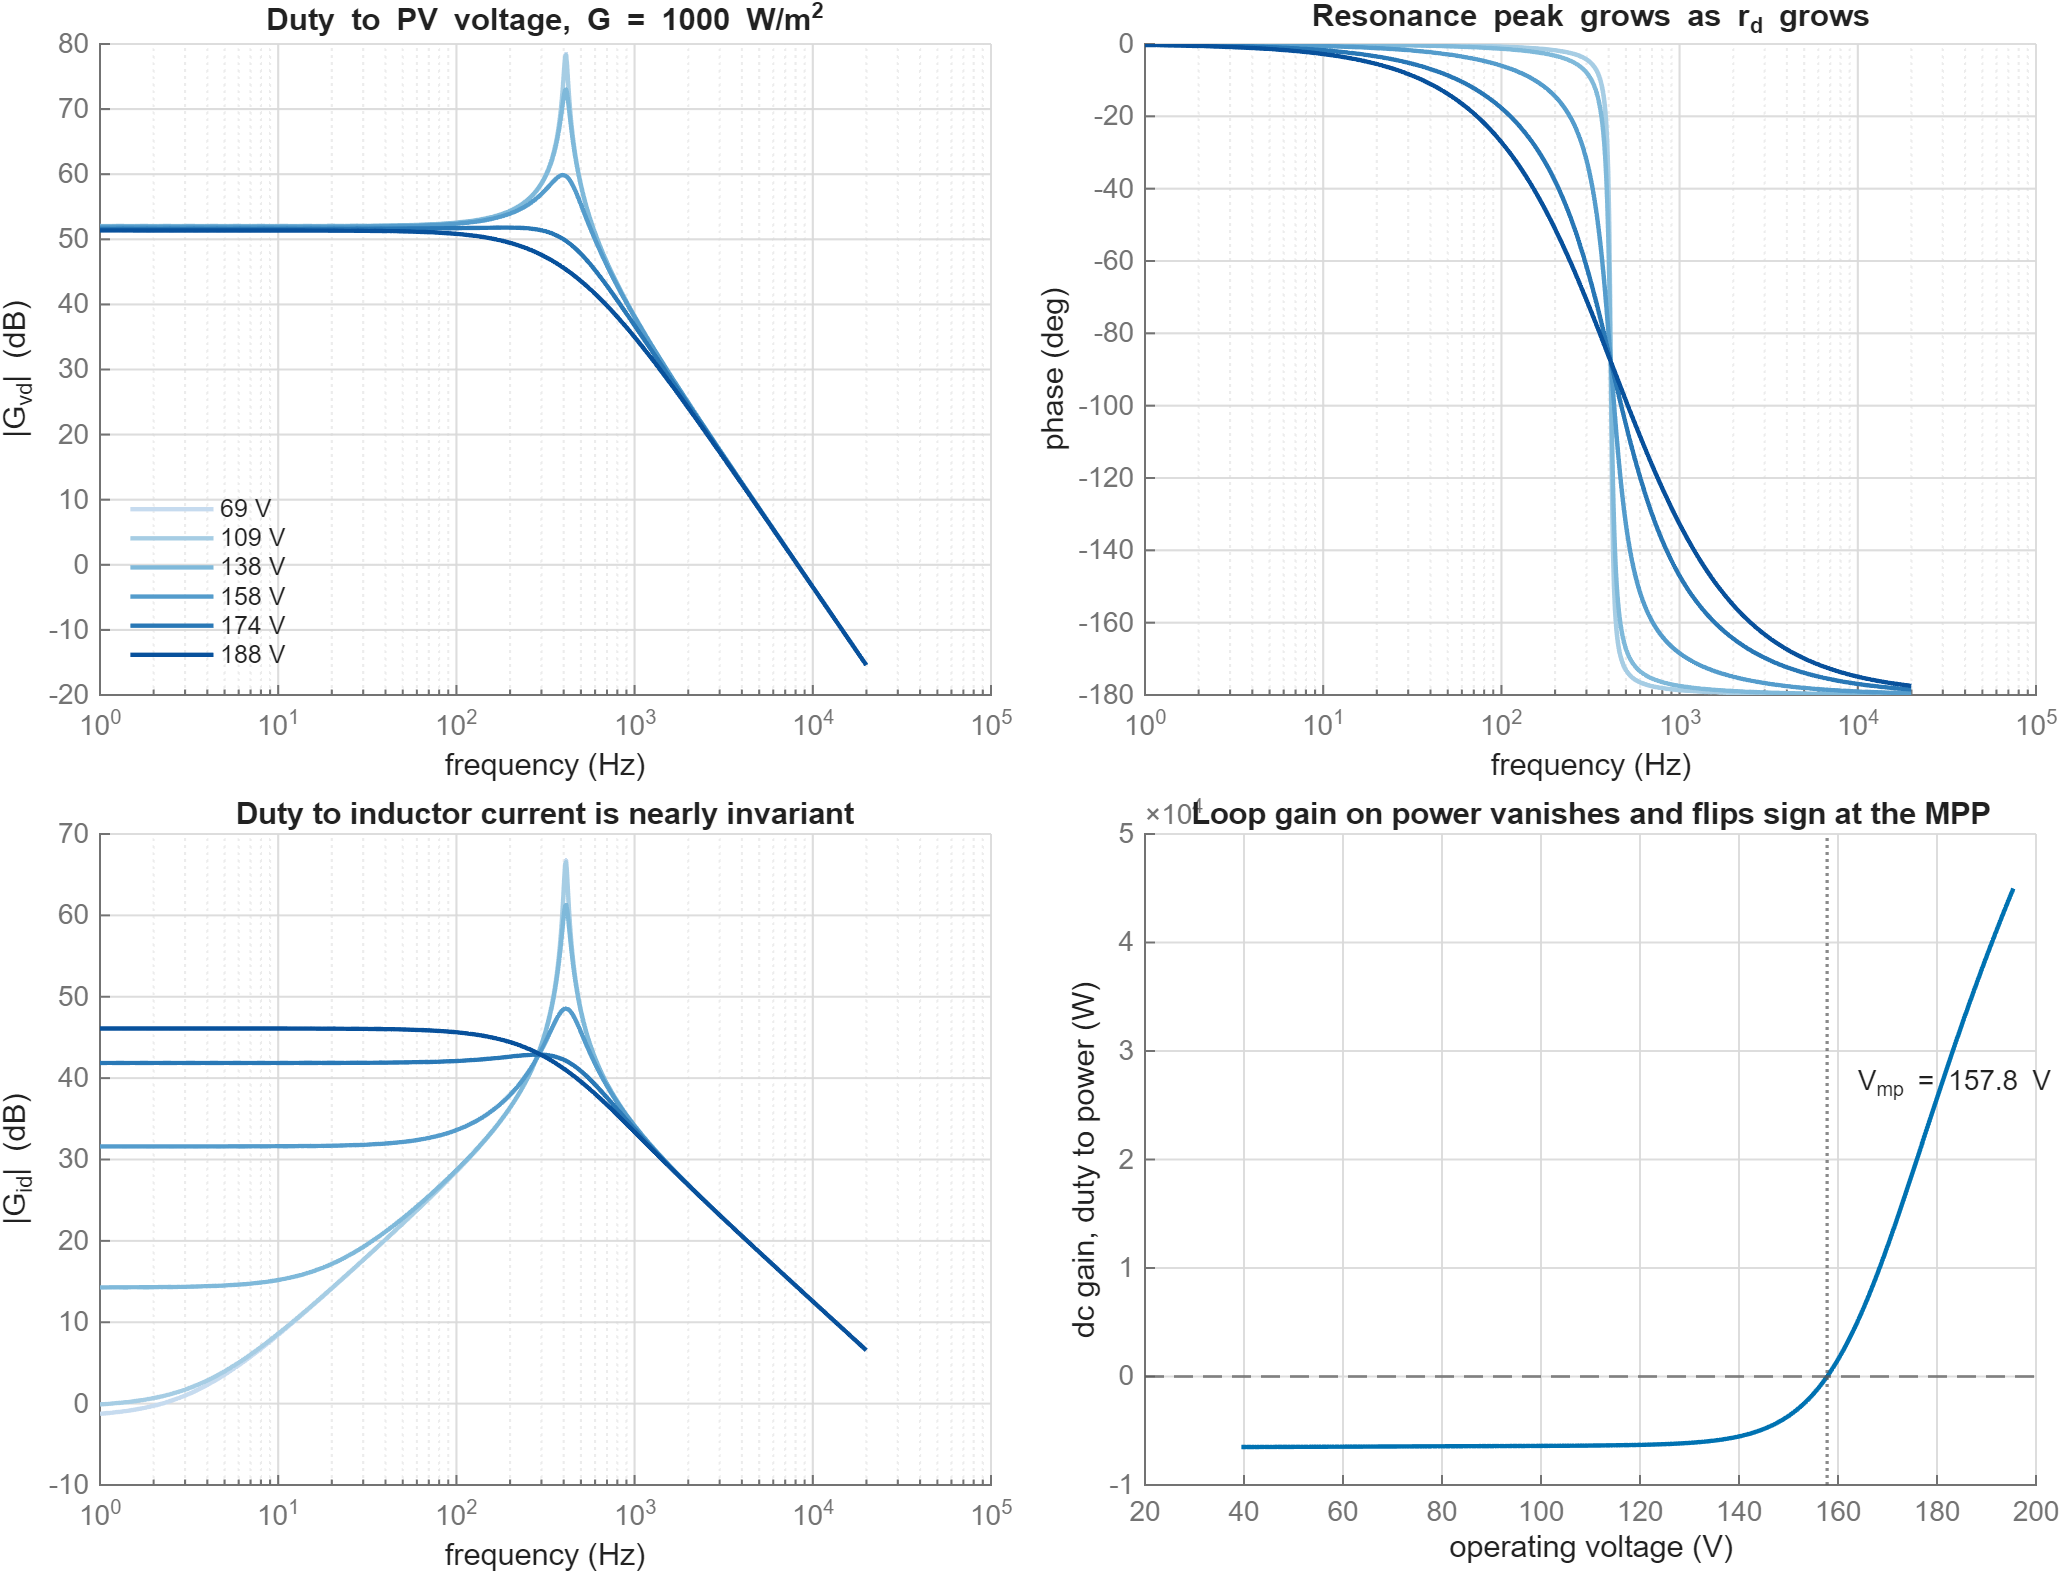
\includegraphics[width=\columnwidth]{figures/s02_plant_frequency_response.png}
\caption{Small-signal plant. Duty to PV voltage at six points along the I--V curve (top); duty to inductor
current, nearly invariant (bottom left); DC gain from duty to power, crossing zero at the MPP (bottom right).}
\label{fig:bode}
\end{figure}

\subsection{Single Loop Versus Cascade}
\label{sec:res-control}
The single loop crosses unity three times, at 56, 130 and \SI{542}{\hertz}, with a peak loop gain of
\SI{43.4}{\decibel}; on the current-source branch its worst phase margin is \SI{1.5}{\degree}
(Table~\ref{tab:pm}). This is structural: keeping $|L|$ below unity through the resonance would push
crossover to a few hertz. The cascade's inner margin lies between \SI{85.0}{\degree} and \SI{85.8}{\degree}
everywhere and its outer margin between \SI{85.3}{\degree} and \SI{122.7}{\degree}. A
\SIrange{140}{165}{\volt} reference step on the nonlinear averaged plant settles to \SI{2}{\percent} in
\SI{11.9}{\milli\second} with no overshoot, and the settled point matches the analytic I--V curve to better
than \SI{0.05}{\percent}. The outer crossover falls from about \SI{223}{\hertz} to \SI{15}{\hertz} near
$\Voc$ (Fig.~\ref{fig:ctrl}); this is benign because that region is far from the MPP and the margin there stays
above \SI{100}{\degree}.

\begin{table}[!t]
\centering
\caption{Worst-Case Phase Margin Along the I--V Curve at 1000~W/m$^2$}
\label{tab:pm}
\footnotesize
\begin{tabular}{@{}rrrrrr@{}}
\toprule
$V$ (V) & $r_d$ ($\Omega$) & $\zeta$ & PI PM ($^\circ$) & Cross. & Cascade PM ($^\circ$) \\
\midrule
69.09 & 482.1 & 0.0234 & 1.46 & 3 & 85.3 \\
108.57 & 417.6 & 0.0240 & 1.57 & 3 & 85.4 \\
128.31 & 182.9 & 0.0299 & 2.61 & 3 & 86.4 \\
138.18 & 77.23 & 0.0444 & 5.14 & 3 & 88.8 \\
148.05 & 27.94 & 0.0884 & 12.91 & 3 & 95.9 \\
157.92 & 10.25 & 0.2068 & 34.50 & 3 & 114.2 \\
167.79 & 4.458 & 0.4463 & 88.62 & 3 & 122.7 \\
177.66 & 2.539 & 0.7600 & 139.8 & 1 & 110.6 \\
187.53 & 1.832 & 1.0350 & 135.4 & 1 & 105.3 \\
\bottomrule
\end{tabular}
\end{table}

\begin{figure}[!t]
\centering
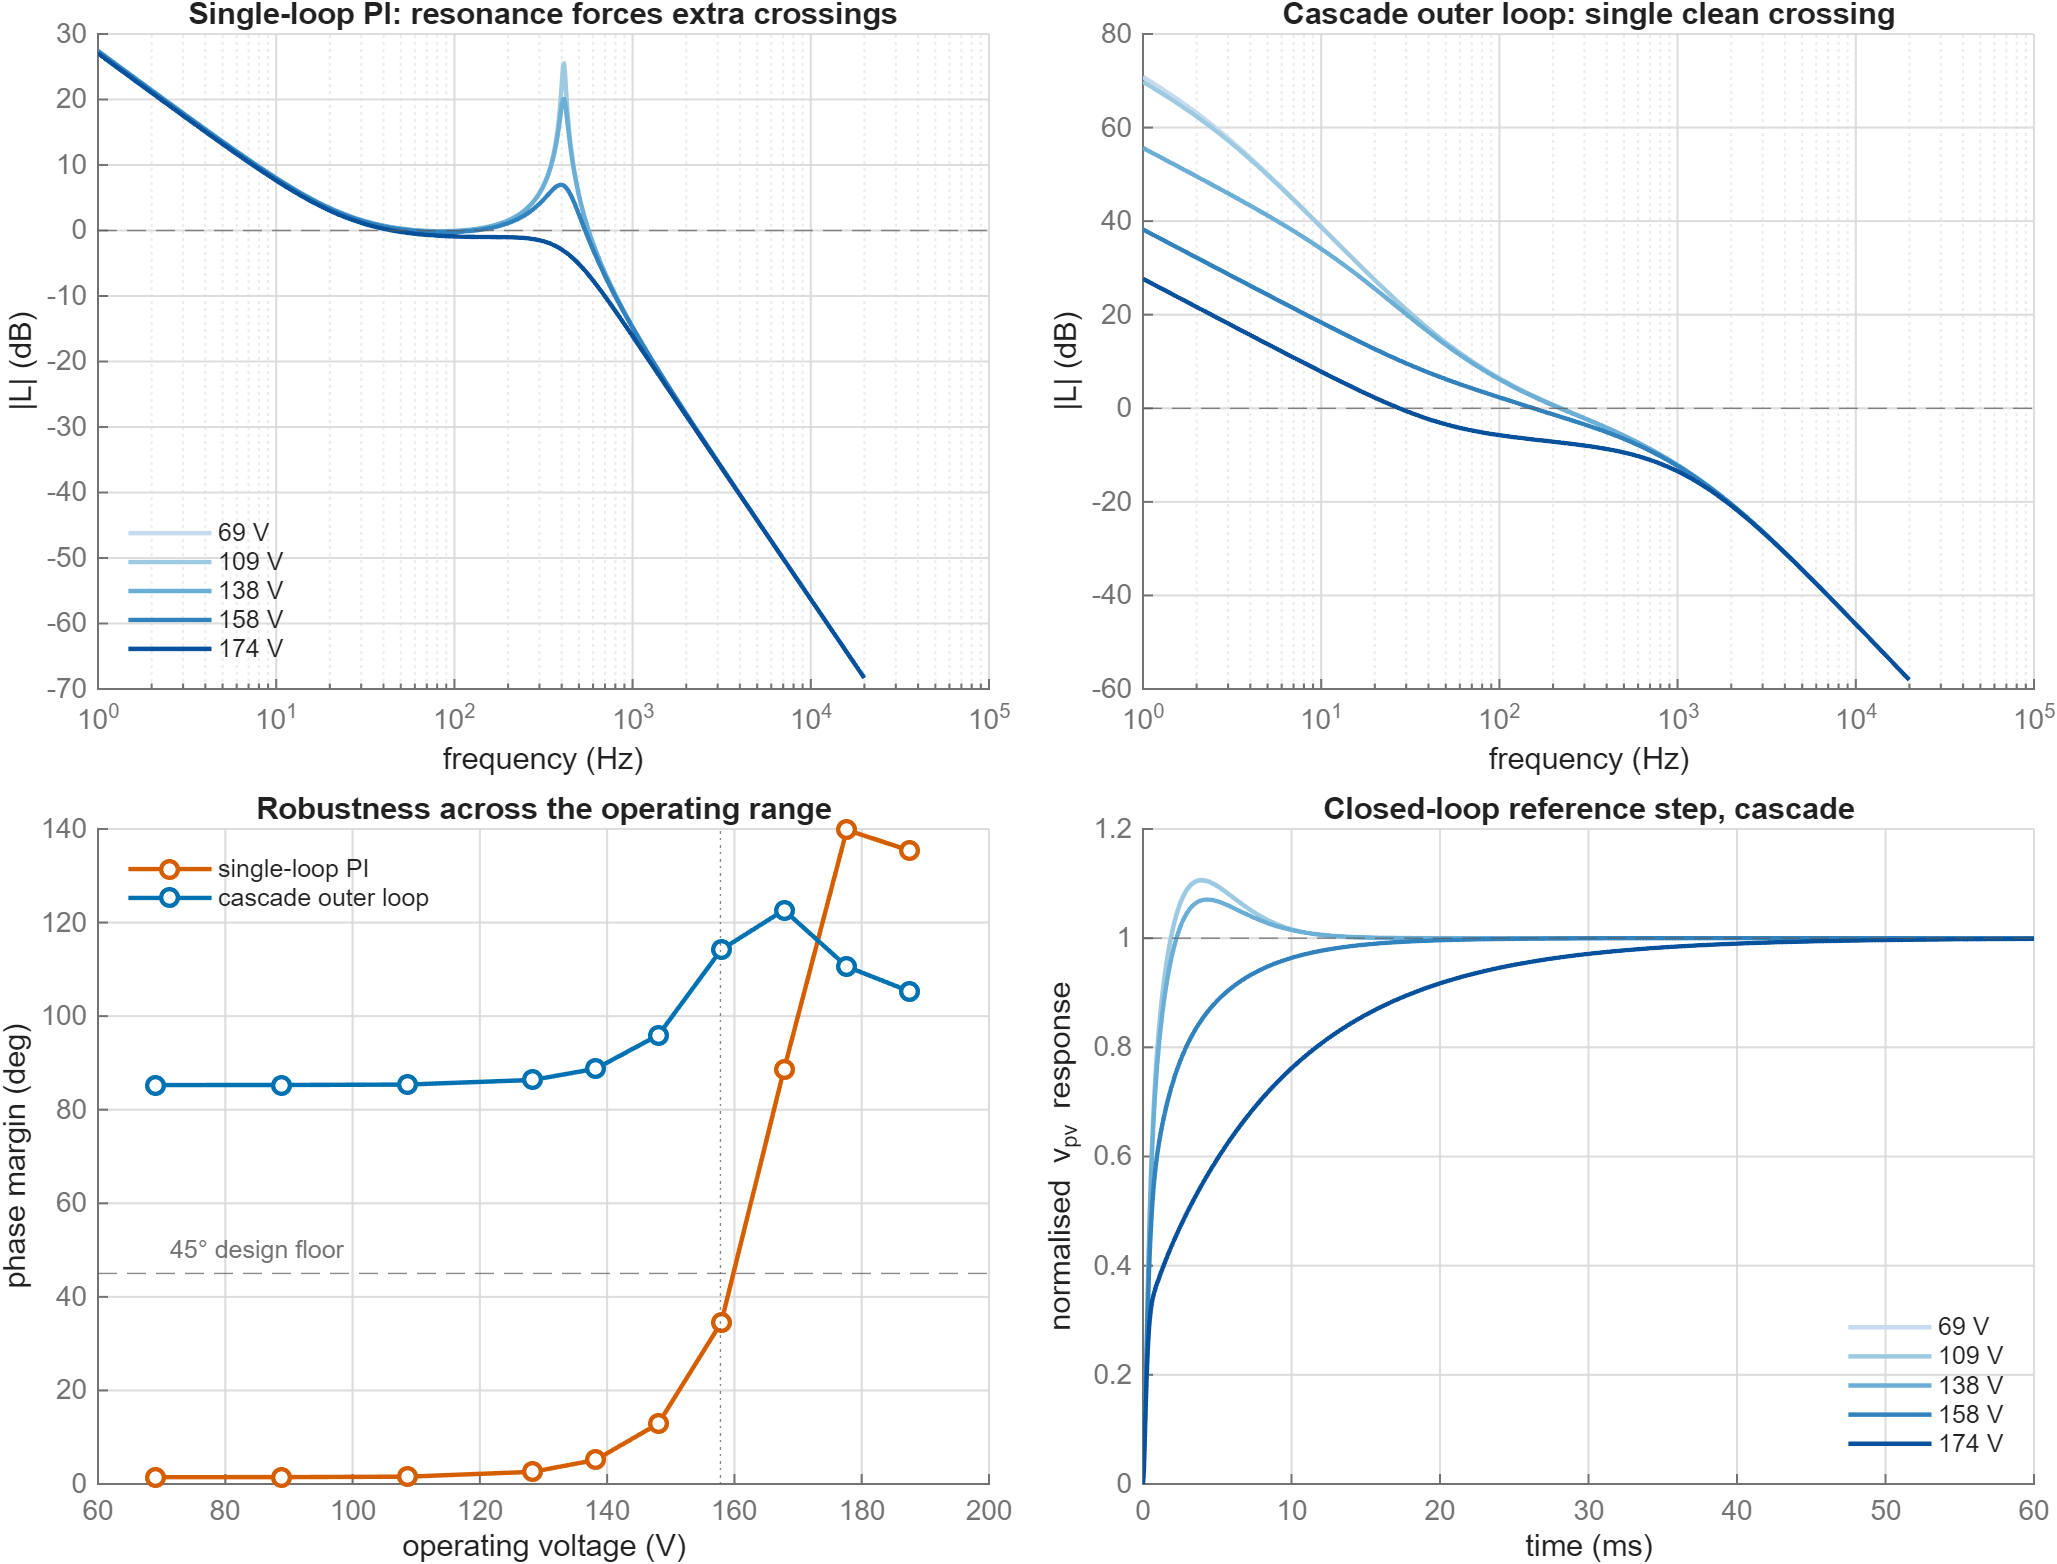
\includegraphics[width=\columnwidth]{figures/s03_control_design.png}
\caption{Single-loop gain magnitude at five operating points (top left), cascade outer loop (top right),
worst-case phase margin against operating voltage (bottom left), and cascade reference steps at five
operating points (bottom right).}
\label{fig:ctrl}
\end{figure}

\subsection{Trackers Under a Step}
\label{sec:res-mppt}
The P\&O limit cycle equals $2\Delta V$ at every step size (1.00 to \SI{11.95}{\volt} for 0.5 to
\SI{6}{\volt} steps), confirming that the voltage loop follows its reference. Cutting acquisition time
eighteenfold, from 1.481 to \SI{0.082}{\second}, costs \SI{0.58}{\percent} of steady-state efficiency. The ESC
gain sweep improves up to $K=20$ (\SI{99.21}{\percent} static efficiency), after which the estimator loop
destabilizes and the excursion jumps from about 6 to \SI{27}{\volt}, as averaging theory predicts; its
estimate settles at \SI{157.75}{\volt} against the true \SI{157.80}{\volt}. Under the step
(Table~\ref{tab:step}, Fig.~\ref{fig:mppt}), variable-step P\&O scores best and ESC worst, penalized only by
its deliberate dither. P\&O and INC are identical, because with the same step and period they compute the
sign of the same quantity.

\begin{table}[!t]
\centering
\caption{Performance Through a 1000 to 500~W/m$^2$ Step}
\label{tab:step}
\footnotesize
\begin{tabular}{@{}lrrrr@{}}
\toprule
Tracker & $\eta$ (\%) & RMS err.\ (V) & Ripple (V) & Deficit (W) \\
\midrule
P\&O, fixed & 99.944 & 1.56 & 3.00 & 182.7 \\
P\&O, variable & \textbf{99.956} & 1.39 & \textbf{0.50} & \textbf{154.6} \\
INC & 99.944 & 1.56 & 3.00 & 182.7 \\
ESC & 99.551 & 4.88 & 5.95 & 194.6 \\
\bottomrule
\end{tabular}
\end{table}

\begin{figure}[!t]
\centering
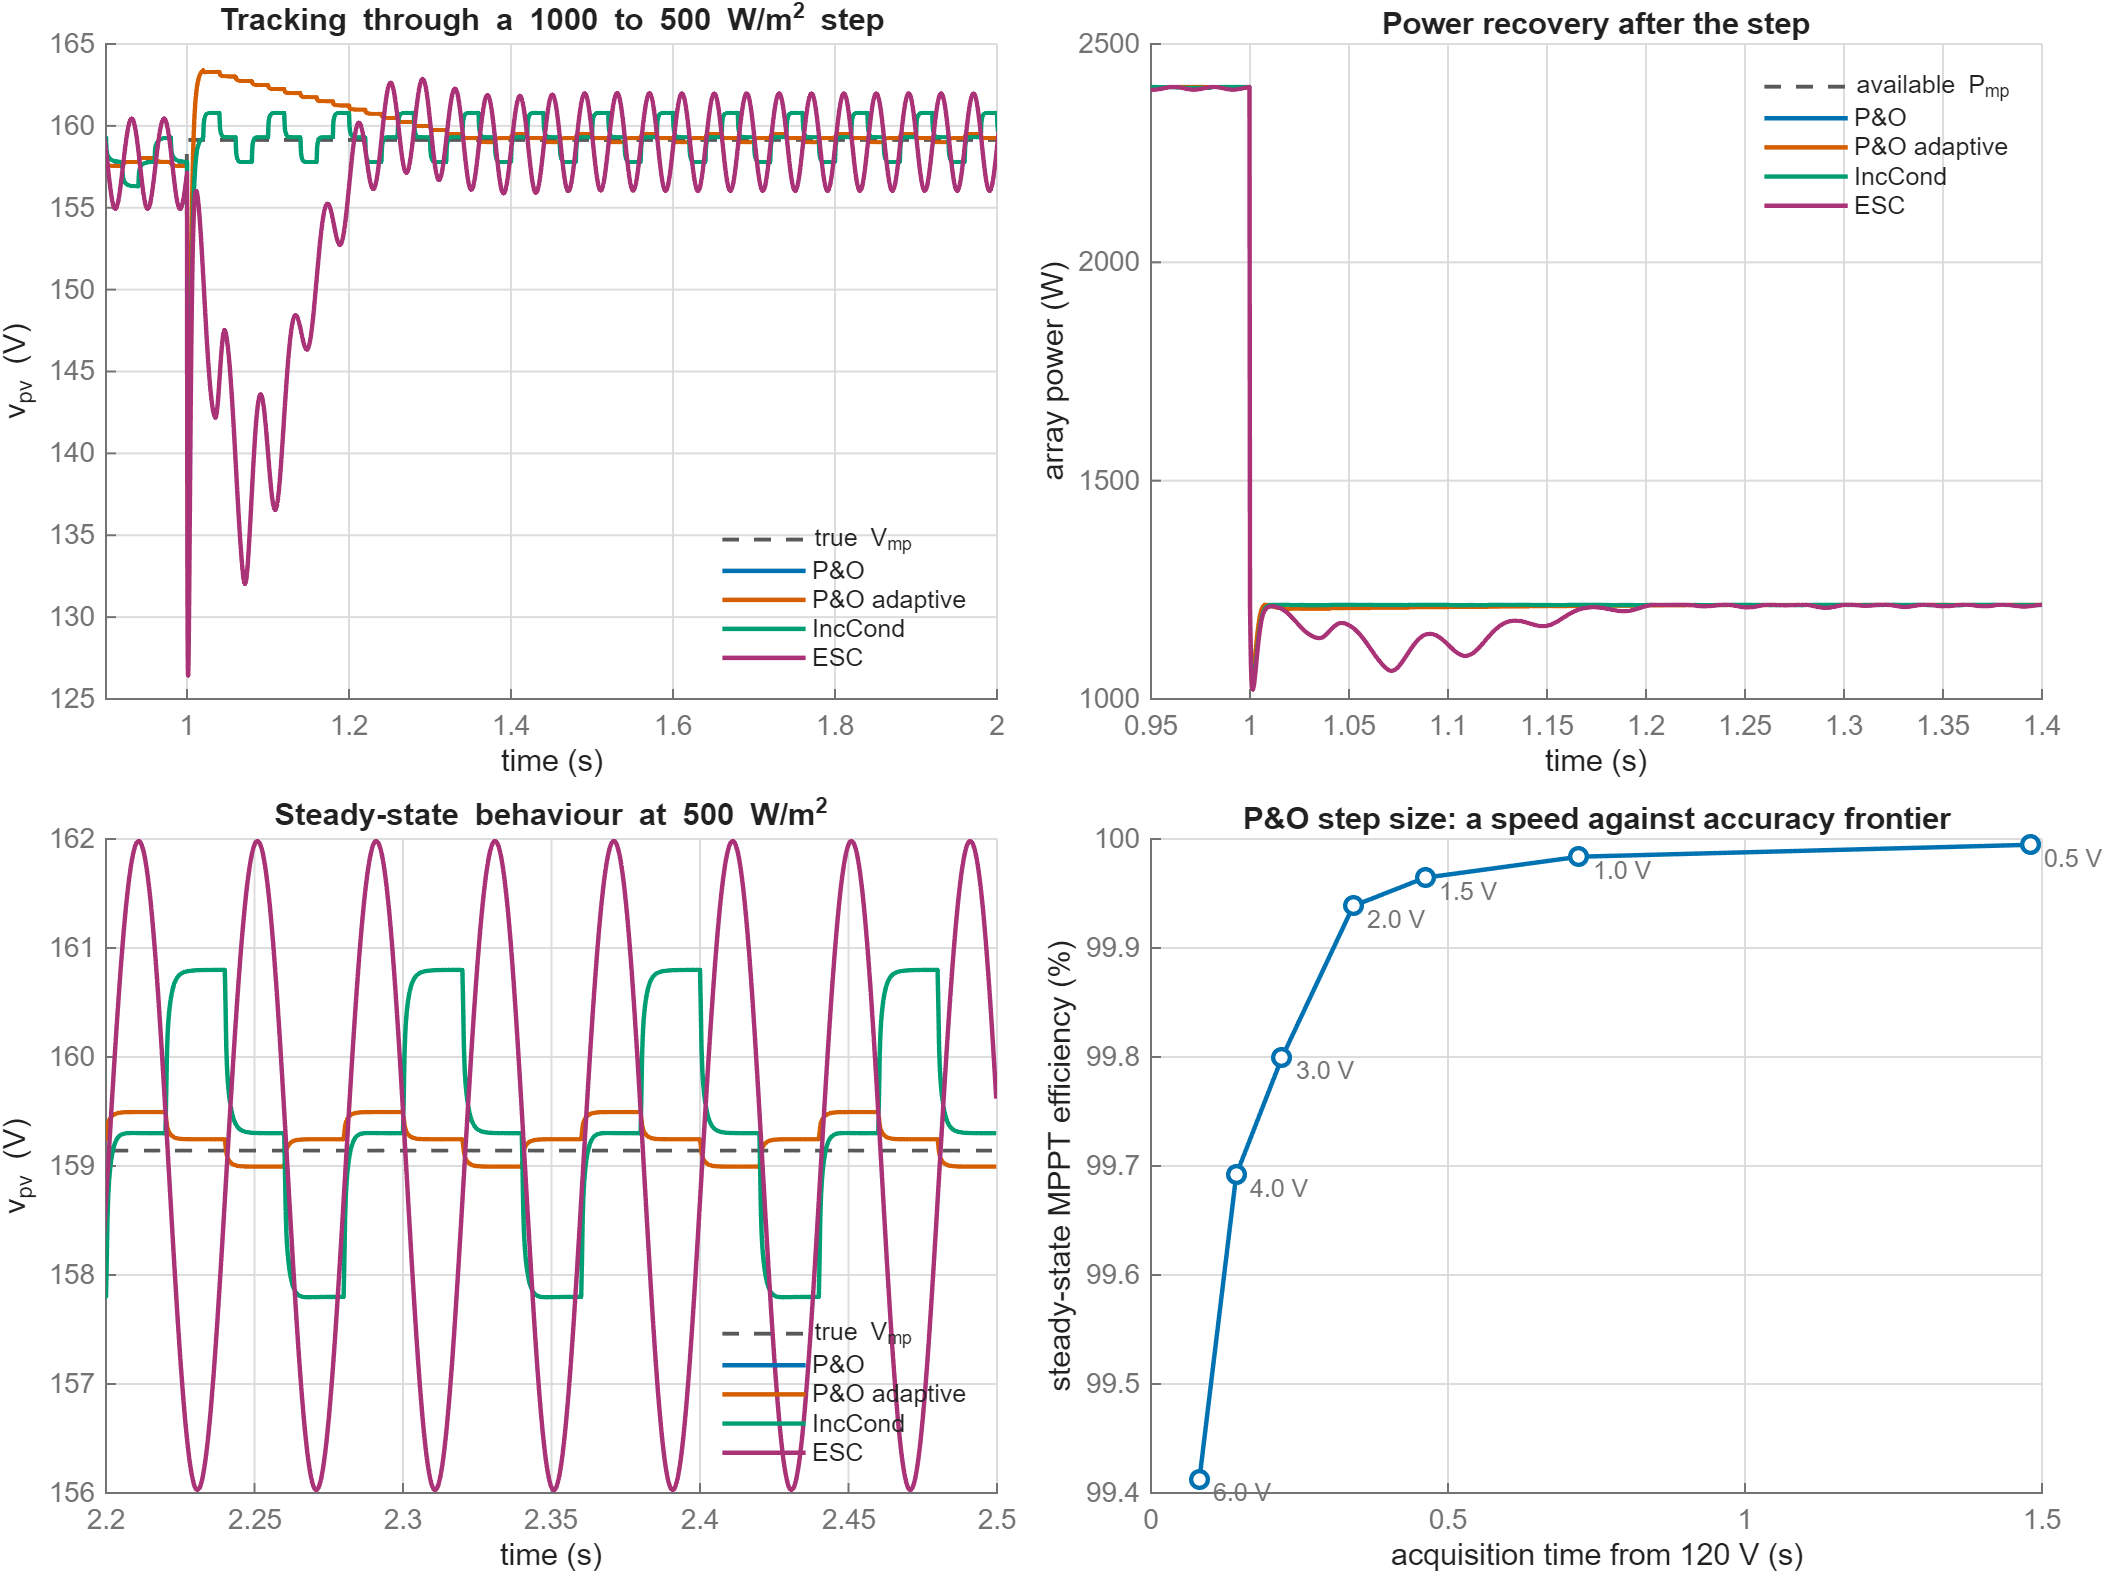
\includegraphics[width=\columnwidth]{figures/s04_mppt_comparison.png}
\caption{Tracker comparison through a \SIrange{1000}{500}{\Wm} step: voltage tracking (top left), power
recovery (top right), steady-state limit cycles and dither (bottom left), and the P\&O speed--accuracy
frontier labeled by step size (bottom right).}
\label{fig:mppt}
\end{figure}

\subsection{Trackers on EN 50530-Style Ramps}
\label{sec:res-bench}
On ramps the ranking inverts (Table~\ref{tab:dyn}, Fig.~\ref{fig:bench}). ESC is rate-independent: an
eightfold change in rate moves its efficiency by \SI{0.001}{\percent}, and its worst shortfall rises only from
6.4 to \SI{8.0}{\watt}. Fixed-step P\&O and INC degrade to 99.483 and \SI{99.458}{\percent} at
\SI{200}{\Wms}, with shortfalls of 116 and \SI{129}{\watt}. Variable-step P\&O collapses to
\SI{93.14}{\percent} at \SI{100}{\Wms} with a \SI{705}{\watt} shortfall, nearly a third of the available
power, as its voltage runs from 158 to below \SI{90}{\volt}.

The mechanism is drift. At \SI{100}{\Wms} and a \SI{20}{\milli\second} period, irradiance rises
\SI{2}{\Wm} between samples, adding about \SI{5}{\watt} at full sun, more than a \SI{1.5}{\volt}
perturbation changes power near the flat peak, so $\Delta P>0$ whichever way the tracker moved~\cite{femia}.
For the variable-step rule this becomes positive feedback: moving away from the peak raises
$|\mathrm{d}P/\mathrm{d}V|$, which enlarges the step, which accelerates the departure. ESC is immune by
construction, because its washout rejects slowly varying power, and a ramp is exactly such a component.

\begin{table}[!t]
\centering
\caption{Dynamic MPPT Efficiency (\%) and Worst Shortfall (W) on Ramps Between 300 and 1000~W/m$^2$}
\label{tab:dyn}
\footnotesize
\setlength{\tabcolsep}{4pt}
\begin{tabular}{@{}lrrrr@{}}
\toprule
Tracker & 25 & 50 & 100 & 200 W/m$^2$/s \\
\midrule
\multicolumn{5}{@{}l}{\emph{Efficiency}} \\
P\&O, fixed & 99.952 & 99.930 & 99.871 & 99.483 \\
P\&O, variable & 99.836 & 98.726 & \textbf{93.141} & 99.652 \\
INC & 99.950 & 99.926 & 99.871 & 99.458 \\
ESC & 99.851 & 99.851 & 99.851 & \textbf{99.850} \\
\midrule
\multicolumn{5}{@{}l}{\emph{Worst shortfall}} \\
P\&O, fixed & 6.24 & 8.21 & 23.37 & 116.17 \\
P\&O, variable & 43.58 & 240.29 & 704.85 & 40.50 \\
INC & 6.84 & 9.15 & 17.93 & 129.26 \\
ESC & \textbf{6.43} & \textbf{6.63} & \textbf{7.04} & \textbf{7.98} \\
\bottomrule
\end{tabular}
\end{table}

\begin{figure}[!t]
\centering
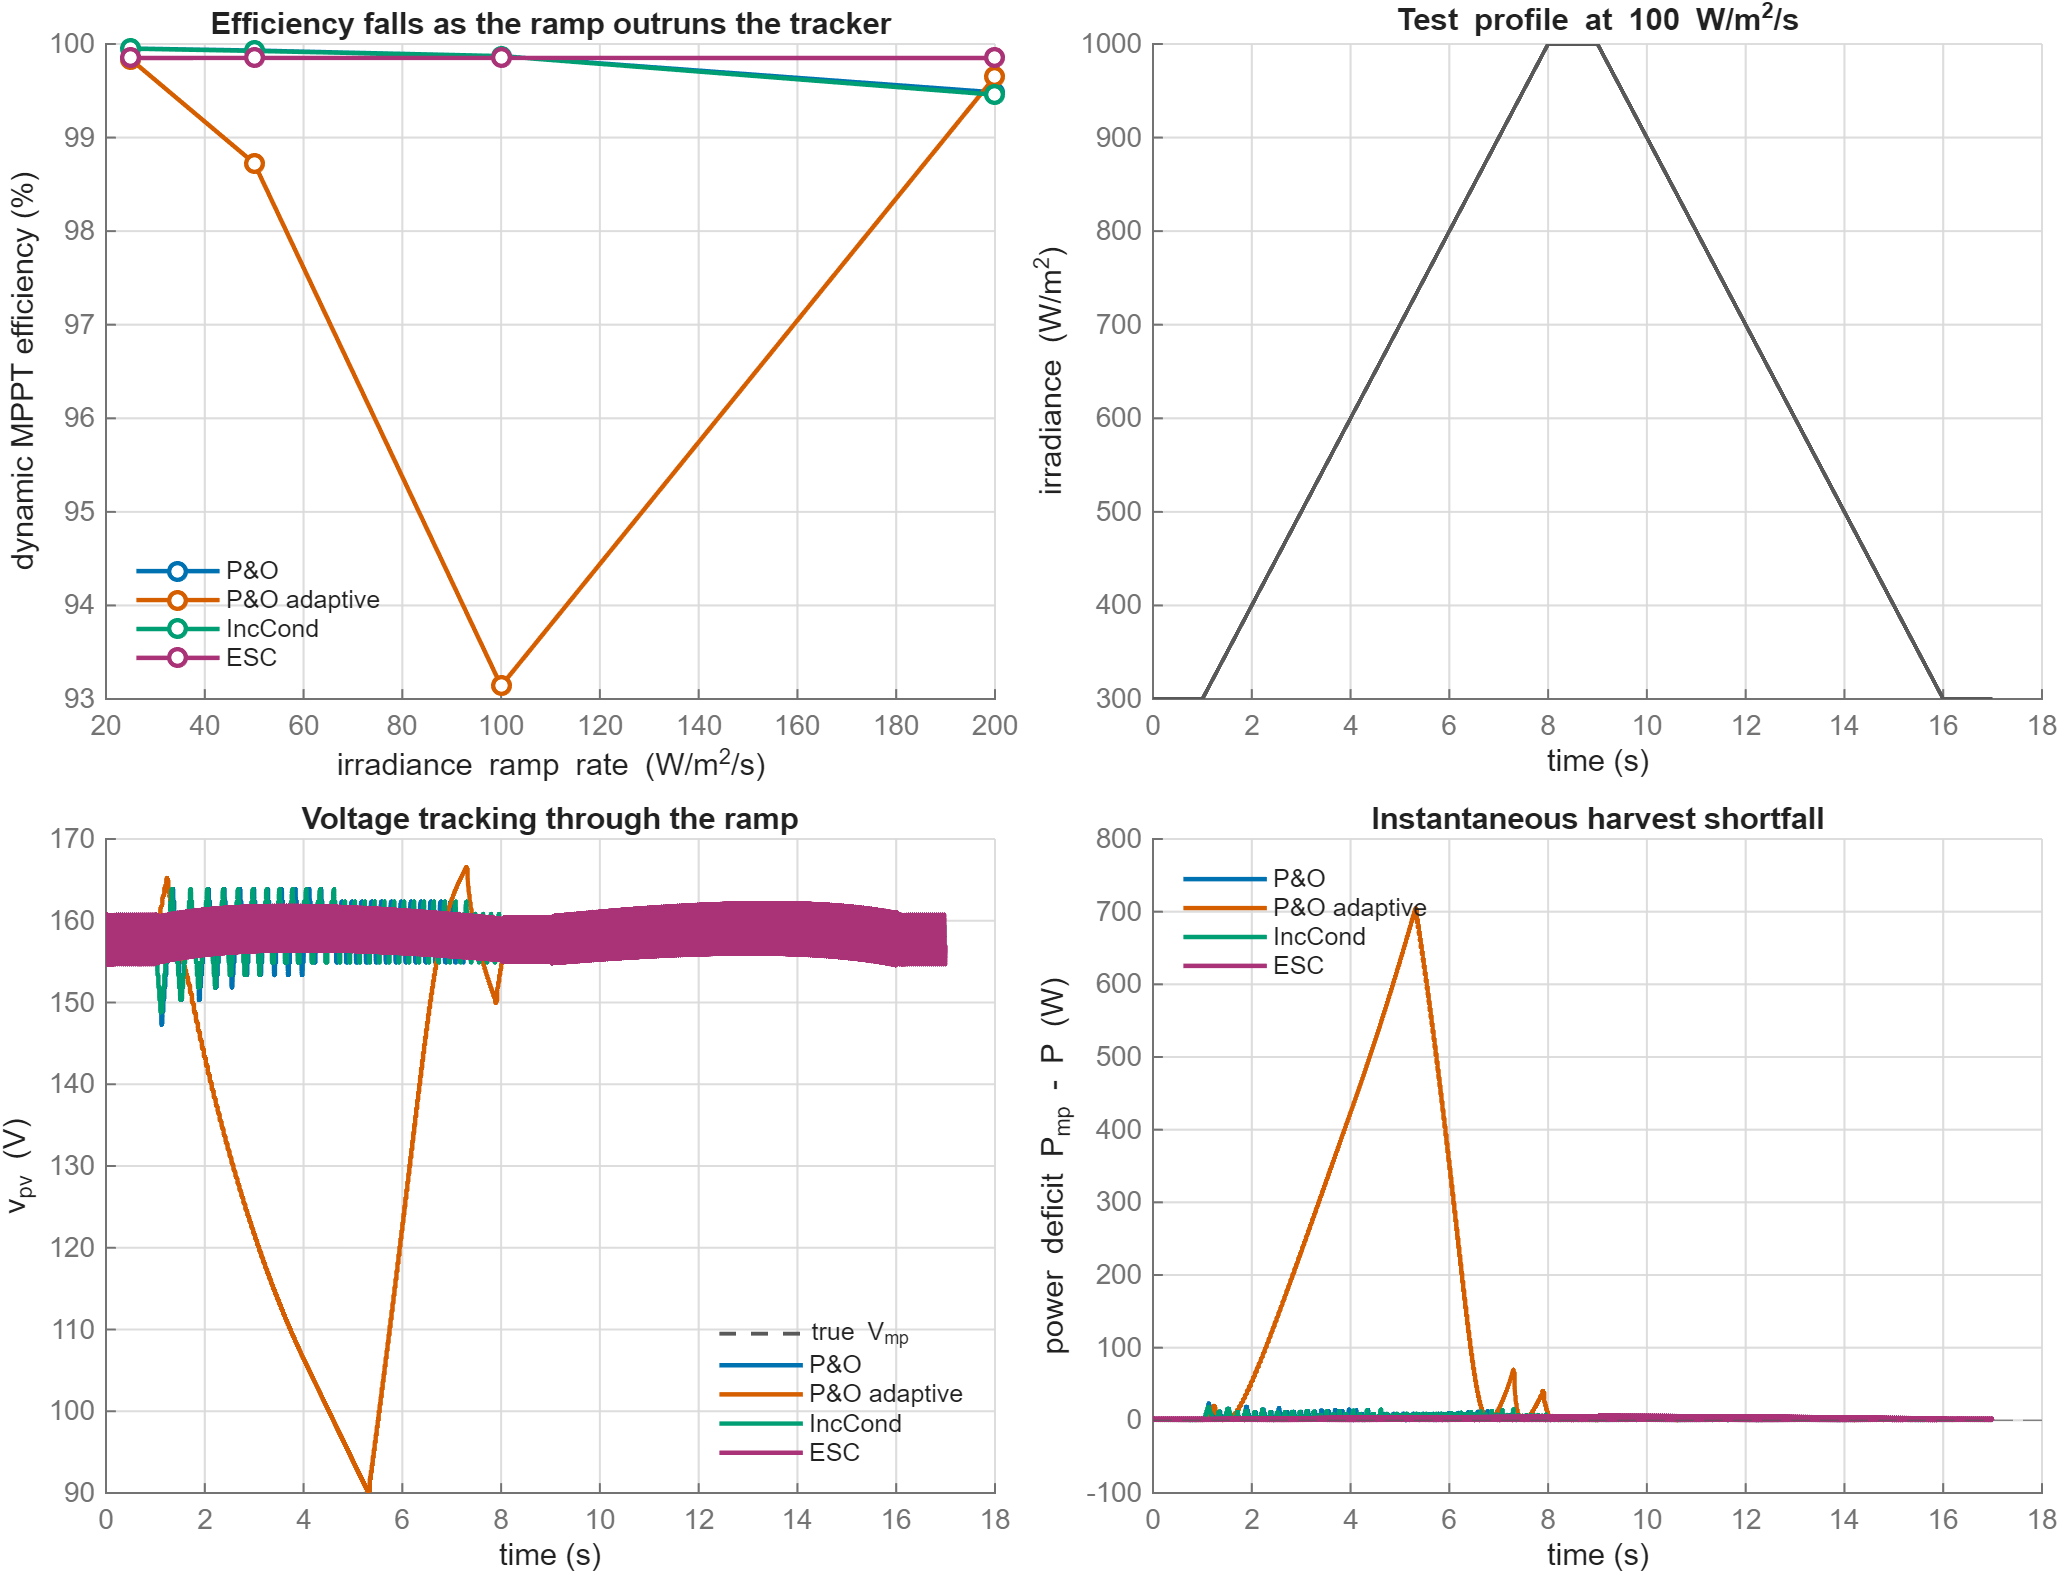
\includegraphics[width=\columnwidth]{figures/s05_dynamic_benchmark.png}
\caption{Dynamic benchmark: efficiency against ramp rate (top left), test profile (top right), voltage
tracking with the variable-step runaway below \SI{90}{\volt} (bottom left), and instantaneous power shortfall
(bottom right).}
\label{fig:bench}
\end{figure}

\subsection{Switched Circuit Validation}
\label{sec:res-switched}
At the predicted duty of 0.6112, open loop, the switched circuit agrees with the averaged model to
\SI{0.23}{\percent} in mean voltage, \SI{0.15}{\percent} in mean current, \SI{1.2}{\percent} in current
ripple and \SI{0.005}{\percent} in mean power (Table~\ref{tab:sw}). The voltage sits slightly high because the
averaged model neglects switch and diode losses. In closed loop with the cascade and P\&O through the step, the
switched circuit harvests \SI{99.93}{\percent}, consistent with \SI{99.94}{\percent} on the averaged model
(Fig.~\ref{fig:sw}).

\begin{table}[!t]
\centering
\caption{Switched Circuit Against Averaged Model at $D=0.6112$, 1000~W/m$^2$}
\label{tab:sw}
\footnotesize
\begin{tabular}{@{}lrrr@{}}
\toprule
Quantity & Switched & Averaged & Difference \\
\midrule
$\vpv$ mean (V) & 158.169 & 157.800 & $+0.234$\,\% \\
$i_L$ mean (A) & 15.198 & 15.220 & $-0.145$\,\% \\
$i_L$ ripple (A) & 3.176 & 3.215 & $-1.23$\,\% \\
$\vpv$ ripple (V) & 0.1946 & 0.2009 & $-3.1$\,\% \\
$P_{\mathrm{pv}}$ mean (W) & 2401.60 & 2401.72 & $-0.005$\,\% \\
\bottomrule
\end{tabular}
\end{table}

\begin{figure}[!t]
\centering
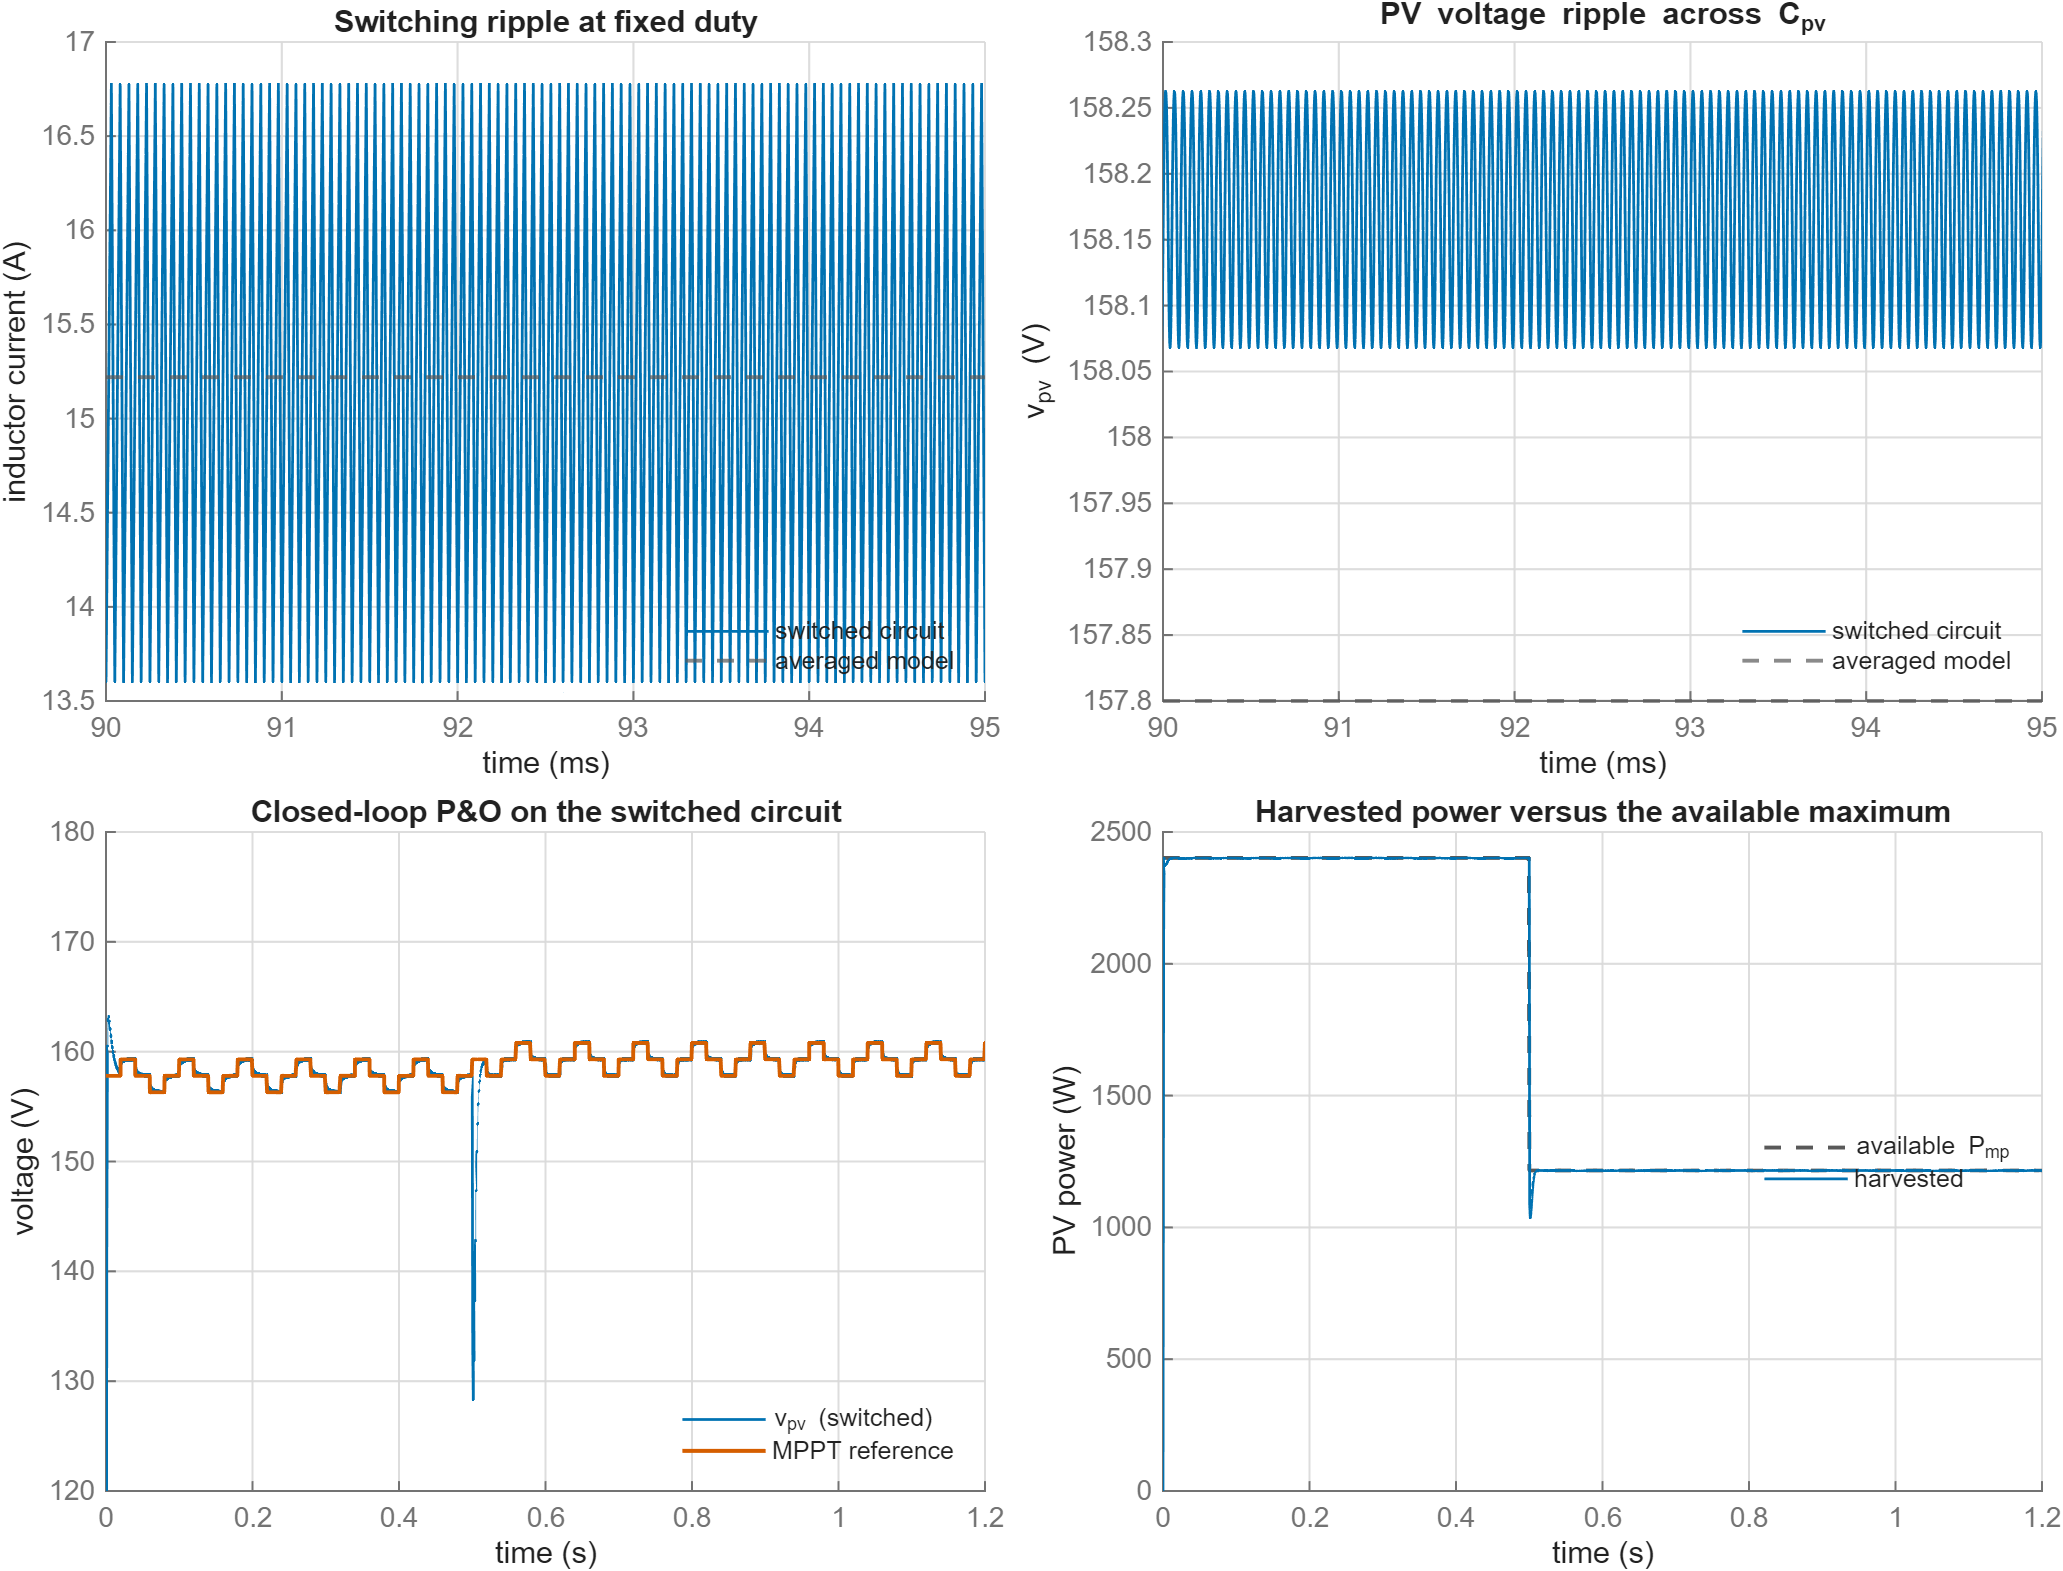
\includegraphics[width=\columnwidth]{figures/s06_switched_validation.png}
\caption{Switched circuit: \SI{20}{\kilo\hertz} ripple in inductor current and PV voltage with the averaged
prediction dashed (top), closed-loop tracking with the P\&O staircase (bottom left), and harvested against
available power through the step (bottom right).}
\label{fig:sw}
\end{figure}

\section{Discussion}
The control framing is predictive. The vanishing power gain explains why trackers estimate gradients; the
dynamic resistance explains where a single loop is fragile; the settling time sets the tracker period; and
frequency separation between dither and disturbance explains why ESC ignores ramps. The best tracker depends on
the site: ESC where irradiance changes fast and often, fixed-step P\&O under stable skies, where it scores
\SI{99.94}{\percent} against \SI{99.55}{\percent}. Adaptation laws are feedback loops and deserve the same
stability analysis as the main loop; a step-only benchmark would have ranked the least robust tracker first.

\emph{Limitations.} Illumination is uniform, so partial shading is untested. Sensing is ideal, which hides the
practical difference between P\&O and INC. The bus is stiff and switches are ideal apart from on-resistance and
forward drop. The EN~50530 profile uses one cycle per slope. No hardware was built; results are validated
against a more detailed simulation, not measurement.

\section{Conclusion}
Treating MPPT as a control problem yields three findings. The array sets its converter's damping, which varies
$44\times$ along one curve, so a single PI loop falls to \SI{1.5}{\degree} of margin while a cascade holds above
\SI{85}{\degree}. The duty-to-power gain vanishes at the optimum, so tracking is gradient estimation, with a
period set by the measured \SI{11.9}{\milli\second} settling time. And on standard ramps ESC holds
\SI{99.85}{\percent} at every rate while the step-test winner falls to \SI{93.14}{\percent}. Future work
covers a drift-free P\&O with an irradiance-change detector, sensor noise models, gain scheduling on the
measured $r_d$, ripple correlation control~\cite{rcc}, partial shading, and a staged hardware build with the
simulated figures as acceptance criteria.

\section*{Data and Code Availability}
The MATLAB library, analysis scripts, Simscape model, 27 unit tests and the source of this paper are available
at \url{https://github.com/riteshroshann/mppt}. The command \texttt{run\_all} rebuilds the model, regenerates
every figure and table, and runs the tests in about \SI{11}{\minute}.

\section*{Acknowledgment}
The authors thank Dr.~Lokendra Singh, Amrita School of Artificial Intelligence, Faridabad, for guidance
throughout this work.

{\footnotesize
\bibliographystyle{IEEEtran}
\bibliography{refs}}

\end{document}
